\documentclass{report}

\usepackage[T1]{fontenc}
\usepackage[utf8]{inputenc}
\usepackage{times}

\usepackage[font=small,labelfont=bf,tableposition=top]{caption}
\usepackage{graphicx}
\usepackage{natbib} 

\usepackage{amsmath}
\usepackage{amsfonts}
\usepackage{amssymb}
\usepackage{color, soul}
\usepackage{hyperref}
\usepackage{algorithmicx}
\usepackage{algpseudocode}
\usepackage{subfigure}
\usepackage{stmaryrd}

\renewcommand{\vec}[1]{\boldsymbol{{#1}}} 
\newcommand{\duesoon}[1]{{\sethlcolor{green}\hl{#1}}}
\usepackage{mathrsfs}


\newtheorem{theorem}{Theorem}
\newtheorem{acknowledgement}[theorem]{Acknowledgement}
\newtheorem{algorithm}[theorem]{Algorithm}
\newtheorem{axiom}[theorem]{Axiom}
\newtheorem{case}[theorem]{Case}
\newtheorem{claim}[theorem]{Claim}
\newtheorem{conclusion}[theorem]{Conclusion}
\newtheorem{condition}[theorem]{Condition}
\newtheorem{conjecture}[theorem]{Conjecture}
\newtheorem{corollary}[theorem]{Corollary}
\newtheorem{criterion}[theorem]{Criterion}
\newtheorem{definition}[theorem]{Definition}
\newtheorem{example}[theorem]{Example}
\newtheorem{exercise}[theorem]{Exercise}
\newtheorem{lemma}[theorem]{Lemma}
\newtheorem{notation}[theorem]{Notation}
\newtheorem{problem}[theorem]{Problem}
\newtheorem{proposition}[theorem]{Proposition}
\newtheorem{remark}[theorem]{Remark}
\newtheorem{solution}[theorem]{Solution}
\newtheorem{summary}[theorem]{Summary}
\newenvironment{proof}[1][Proof]{\textbf{#1.} }{\ \rule{0.5em}{0.5em}}

\newtheorem{guess}{Definition}
\newcommand{\comment}[1] {}
\newcommand{\Norder} {N}
\newcommand{\order}{\mathcal{O}}
\newcommand{\Npoints} {N_p}
\newcommand{\Nfaces} {N_{f}}
\newcommand{\Nelements} {N_e}

\newcommand{\eps}{\varepsilon}
\newcommand{\Dweak}{\wt{D}}
\newcommand{\diff}[2] {\frac{\partial #1}{\partial #2}}
\newcommand{\dxx}[2] {\frac{\partial^2 #1}{\partial {#2}^2}}
\newcommand{\difft}[2] {\frac{d #1}{d #2}}
\newcommand{\dxxt}[2] {\frac{d^2 #1}{d {#2}^2}}
\newcommand{\lagrange}[1] {\frac{d #1}{dt}}
\newcommand{\lebesgue}{\parallel I \parallel}
\newcommand{\polysp}{\mathcal{P}_N}
\newcommand{\laplacian}{\nabla^2}
\newcommand{\divergence}{\nabla \cdot}
\newcommand{\inte}{\int_{\mbox{\footnotesize ${\Omega_e}$}}}
\newcommand{\intb}{\int_{\mbox{\footnotesize ${\Gamma_e}$}}}
\newcommand{\intce}{\int_{\mbox{\footnotesize ${\widehat{\Omega}_e}$}}}
\newcommand{\intcb}{\int_{\mbox{\footnotesize ${\widehat{\Gamma}_e}$}}}
\newcommand{\intg}{\int_{\mbox{\footnotesize ${\Omega}$}}}
\newcommand{\intgb}{\int_{\mbox{\footnotesize ${\Gamma}$}}}
\newcommand{\intv}{\int_{\mbox{\footnotesize ${\sigma}$}}}
\newcommand{\sumv}{\sum_{K=1}^{N_{\mathrm{lev}}}}
\newcommand{\sumk}{\sum_{L=1}^{K}}
\newcommand{\sumN}{\sum_{i=1}^{N+1}}
\newcommand{\half}{\frac{1}{2}}
\newcommand{\inti}{\int_{\mbox{\footnotesize\sf I}}}
\newcommand{\intbd}{\oint_{\mbox{\footnotesize ${\delta}$\sf D}}}
\newcommand{\intbi}{\oint_{\mbox{\footnotesize ${\delta}$\sf I}}}
\newcommand{\ldnorm}[1]{\left\| #1 \right\|_{\mbox{\footnotesize \sf D}} }
\newcommand{\lonorm}[1]{\left\| #1 \right\|_{\Omega}}
\newcommand{\spc}[1]{\mbox{\sf #1}}
\newcommand{\ope}[1]{{\cal #1}}
\newcommand{\mt}[1]{{\rm #1}}
\newcommand{\dis}{\displaystyle}
\newcommand{\ve}{\varepsilon}
\newcommand{\ov}{\overline}
\newcommand{\wt}{\widetilde}
\newcommand{\wh}{\widehat}
\newcommand{\Dhat}{\widehat{D}}
\newcommand{\be}{\begin{equation}}
\newcommand{\ee}{\end{equation}}
\newcommand{\bea}{\begin{eqnarray*}}
\newcommand{\eea}{\end{eqnarray*}}
\newcommand{\Jace}{J^{(e)}}
\newcommand{\Jacl}{J^{(l)}}
\def\bepsilon{\mbox{\boldmath $\epsilon $}}
\def\bpsi{\mbox{\boldmath $\psi $}}
\def\bphi{\mbox{\boldmath $\phi $}}
\def\bmu{\mbox{\boldmath $\mu $}}
\def\Et{ \tilde{E} }
\def\Ht{ \tilde{H} }
\def\sdot{ \dot{\sigma} }

\newcommand{\fstar}{f^{(*)}}

\DeclareMathOperator{\Span}{span}
\DeclareMathOperator{\Dim}{dim}

\newcommand{\polyquad}{\mathcal{Q}_{N}}
\newcommand{\polyP}{\mathcal{P}_{N}}
\newcommand{\polyPnpm}{\mathcal{P}_{(N+M)}}
\newcommand{\polyPd}{\mathcal{P}_{d}}
\newcommand{\polyPnm}{\mathcal{P}_{N,M}}
\newcommand{\polyPn}{\mathcal{P}_{N,0}}
\newcommand{\transpose}{^{\mathcal{T}}}

\newcommand{\vecQ}{\vec{Q}}
\newcommand{\vecQe}{\vec{Q}^{(e)}}
\newcommand{\vecFe}{\vec{\mathcal{F}}^{(e)}}
\newcommand{\statevec}{\vec{Y}}
\newcommand{\statevecN}{\vec{Y}_N^{(e)}}
\newcommand{\statestage}{\vec{\mathcal{Y}}}
\newcommand{\Ftensor}{\vec{F}(\qvector)}
\newcommand{\FtensorN}{\vec{F}\left( \qvectorN \right)}
\newcommand{\FtensorStar}{\vec{F}\left( \qvector_N^{(e,k)} \right)}
\newcommand{\Svector}{S(\qvector)}
\newcommand{\SvectorN}{S \left( \qvectorN \right)}
\newcommand{\qref}{\vec{q}_0}
\newcommand{\qvectorb}{\vec{q}_b}
\newcommand{\qtt}{\vec{q}_{tt}}
\newcommand{\qhat}{\widehat{\vec{q}}}
\newcommand{\qhatb}{\widehat{\vec{q}}_b}
\newcommand{\qelem}{q^{(e)}}
\newcommand{\rhoref}{\rho_0}
\newcommand{\piref}{\pi_0}
\newcommand{\Thetaref}{\Theta_0}
\newcommand{\Gref}{G_0}
\newcommand{\Tref}{T_0}
\newcommand{\thetaref}{\theta_0}
\newcommand{\Pref}{{P}_0}
\newcommand{\Eref}{{E}_0}
\newcommand{\Href}{{h}_0}
\newcommand{\rhohat}{\widehat{\rho}}
\newcommand{\pihat}{\widehat{\pi}}
\newcommand{\Phat}{\widehat{P}}
\newcommand{\uvechat}{\widehat{{\mbox{\boldmath$u$\unboldmath}}}}
\newcommand{\uhathat}{\widehat{\widehat{{\mbox{\boldmath$u$\unboldmath}}}}}
\newcommand{\Uhat}{\widehat{{\mbox{\boldmath$U$\unboldmath}}}}
\newcommand{\Uhathat}{\widehat{\widehat{{\mbox{\boldmath$U$\unboldmath}}}}}
\newcommand{\thetahat}{\widehat{\theta}}
\newcommand{\Thetahat}{\widehat{\Theta}}
\newcommand{\Ehat}{\widehat{E}}
\newcommand{\uhat}{\widehat{u}}
\newcommand{\vhat}{\widehat{v}}
\newcommand{\what}{\widehat{w}}
\newcommand{\pitt}{\pi_{tt}}
\newcommand{\rhott}{\rho_{tt}}
\newcommand{\Ett}{E_{tt}}
\newcommand{\Utt}{\vec{U}_{tt}}
\newcommand{\uvectt}{\vec{u}_{tt}}
\newcommand{\utt}{u_{tt}}
\newcommand{\vtt}{v_{tt}}
\newcommand{\wtt}{w_{tt}}
\newcommand{\Ptt}{P_{tt}}
\newcommand{\vecPtt}{\vec{P}_{tt}}
\newcommand{\Thetatt}{\Theta_{tt}}
\newcommand{\thetatt}{\theta_{tt}}
%Projector Matrices
\newcommand{\projmatrix}{\vec{\mathcal{P}}}
\newcommand{\qmatrix}{\vec{\mathcal{Q}}}
\newcommand{\pcmatrix}{\vec{\mathcal{P}}_C}
\newcommand{\Cmatrix}{\left(\vec{\mathcal{C}}^{(e,f)}\right)\transpose}
\newcommand{\Dmatrix}{\vec{D}^{(e)}}
\newcommand{\Dwmatrix}{\wt{\vec{D}}^{(e)}}
\newcommand{\Mmatrix}{M^{(e)}}
\newcommand{\Fmatrix}{\vec{F}^{(e,l)}}
\newcommand{\Gmatrix}{\mathcal{G}}
\newcommand{\Umatrix}{\mathcal{U}^{(e,f)}}
\newcommand{\amatrix}{\vec{\mathcal{A}}}
\newcommand{\rmatrix}{\vec{\mathcal{R}}}
%Vectors
\newcommand{\nvector}{\wh{\vec{n}}_{\Gamma}}
\newcommand{\nhat}{\wh{\vec{n}}}
\newcommand{\ivector}{\wh{\vec{i}}}
\newcommand{\jvector}{\wh{\vec{j}}}
\newcommand{\kvector}{\wh{\vec{k}}}
\newcommand{\rvector}{\wh{\vec{r}}}
\newcommand{\svector}{\wh{\vec{s}}}
\newcommand{\tvector}{\wh{\vec{t}}}
\newcommand{\vvector}{\wh{\vec{v}}}
\newcommand{\Qvector}{\vec{Q}}
%Vectors
\newcommand{\ur}{{u}^{(r)}}
\newcommand{\us}{{u}^{(s)}}
\newcommand{\ut}{{u}^{(t)}}
\newcommand{\urtt}{{u}_{tt}^{(r)}}
\newcommand{\ustt}{{u}_{tt}^{(s)}}
\newcommand{\uttt}{{u}_{tt}^{(t)}}
\newcommand{\urhat}{\widehat{u}^{(r)}}
\newcommand{\ushat}{\widehat{u}^{(s)}}
\newcommand{\uthat}{\widehat{u}^{(t)}}
%Other Operators
\newcommand{\grad}{\vec{\nabla}}
\newcommand{\Grad}{\vec{\nabla}}
\newcommand{\Dskew}{\mathcal{D}}

\def\bepsilon{\mbox{\boldmath $\epsilon $}}
\def\bpsi{\mbox{\boldmath $\psi $}}
\def\bphi{\mbox{\boldmath $\phi $}}
\def\bmu{\mbox{\boldmath $\mu $}}
\def\Et{ \tilde{E} }
\def\Ht{ \tilde{H} }
\def\sdot{ \dot{\sigma} }
%\renewcommand{\thetable}{\Roman{table}}
%\renewcommand{\thefigure}{\arabic{figure}}

%\DeclareMathOperator{\Span}{span}
%\DeclareMathOperator{\Dim}{dim}

%Editing Commands
\newcommand{\here}{ \textcolor{red}{YOU ARE HERE}}

%Time-Integration
\newcommand{\dt}{{\Delta t}}
\newcommand\ST{\rule[-0.75em]{0pt}{2em}}
\newcommand{\Sfunction}{\mathcal{S}}
\newcommand{\Lfunction}{\mathcal{L}}
\newcommand{\Nfunction}{\mathcal{N}}

%DG Operators
\newcommand{\average}[1]{ \left\{ #1 \right\} }
\newcommand{\jump}[1]{ \llbracket #1 \rrbracket }

%HDG Matrices
\newcommand{\CCmatrix}{\mathcal{C}^{(e,k)}}
\newcommand{\Jmatrix}{\mathcal{J}^{(e,k)}}
\newcommand{\DDmatrix}{\wt{D}^{(e)}}
\newcommand{\SSvector}{\mathcal{S}(q)}
\newcommand{\cghdg}{cg\underline{\hspace{0.15cm}}to\underline{\hspace{0.15cm}}hdg}
%\newcommand{\ul}{\underline{\hspace{0.15cm}}}
\newcommand{\RRmatrix}{\mathcal{R}}

%Clima specific variables
\newcommand{\etotal}{e^{\mathrm{tot}}}
\newcommand{\Etotal}{E^{\mathrm{tot}}}
\newcommand{\Fvector}{\vec{\mathcal{F}}}
\newcommand{\Pvector}{\vec{\mathcal{P}}}
\newcommand{\Fadv}{\vec{\mathcal{F}}^{\mathrm{adv}}}
\newcommand{\Fndf}{\vec{\mathcal{F}}^{\mathrm{ndf}}}
\newcommand{\Fdiff}{\vec{\mathcal{F}}^{\mathrm{diff}}}
\newcommand{\Tvector}{\vec{\mathcal{T}}}
\newcommand{\Source}{\vec{\mathcal{S}}}

\newcommand{\fxg}[1]{\textcolor{cyan}{FXG: #1}}


\usepackage[inline]{enumitem}


\title{CLIMA Atmosphere Model} 
\author{ }

\begin{document}

\maketitle
\tableofcontents

\chapter{Thermodynamics of Moist Air}\label{s:thermodynamics}

The thermodynamics of moist air is often subject to empirical approximations, which usually are opaque, internally inconsistent, and/or inconsistent across model components. For example, microphysical process models often use different approximations for thermodynamic quantities such as saturation vapor pressures than the dynamical core. The often bewildering array of approximations makes it difficult to achieve global conservation, e.g., of energy, and it complicates the use of models for other planetary atmospheres, with different thermodynamic parameters. 

Here we employ one consistent set of thermodynamic approximations for all model components. These result in straightforward, easily adaptable, and relatively accurate expressions for thermodynamic quantities, including closed-form expressions of saturation vapor pressures in terms of thermodynamic parameters. The key to thermodynamic consistency at reasonable accuracy is to take the specific heat capacities of the constituents of moist air (dry air, water vapor, liquid water, and ice) to be constant. All other thermodynamic quantities can then be derived \citep[cf.][]{Romps08a,Marquet16a}. 

\section{Working Fluid and Equation of State}

The working fluid of the atmosphere model is moist, potentially cloudy air, considered to be an ideal mixture of dry air, water vapor, and condensed water (liquid and ice) in clouds. Dry air and water vapor are taken to be ideal gases. The specific volume of the cloud condensate is neglected relative to that of the gas phases (it is a  factor $10^{3}$ less than that of the gas phases). All phases are assumed to have the same temperature, and are advected with the same velocity. The cloud condensates may be sedimenting relative to the gas phases, but slowly enough to be in thermal equilibrium with the surrounding fluid. However, the condensates do not need to be in thermodynamic equilibrium with the other fluid constituents; out-of-equilibrium phases such as supercooled liquid can exist. Falling condensate (precipitation) is not considered part of the working fluid because it generally cannot be assumed to be in thermal equilibrium with the surrounding fluid; it is treated separately.

The density of the moist air is denoted by $\rho$. We use the following notation for the mass fractions of the moist air mixture (mass of a constituent divided by the total mass of the working fluid):
\begin{itemize}
\item $q_d$: dry air mass fraction,
\item $q_v$: water vapor specific humidity,
\item $q_l$: liquid water specific humidity,
\item $q_i$: ice specific humidity,
\item $q_c = q_l + q_i$: condensate specific humidity,
\item $q_t = q_v + q_c$: total specific humidity.
\end{itemize}
Because this enumerates all constituents of the working fluid, we have $q_t + q_d = 1$. In Earth's atmosphere, the water vapor specific humidity $q_v$ generally dominates the total specific humidity $q_t$ and is usually $\order(10^{-2})$ or smaller; the condensate specific humidity is typically $\order(10^{-4})$. Hence, water is a trace constituent of the atmosphere, and only a small fraction of atmospheric water is in condensed phases. 

The pressure $p$ of the working fluid is the sum of the partial pressures of dry air and water vapor, both taken to be ideal gases. Neglecting the volume of the condensed phases (but not their masses), this gives $p = \rho (R_d q_d + R_v q_v) T$, where $R_d$ is the specific gas constant of dry air, and $R_v$ is the specific gas constant of water vapor. Since $q_d = 1-q_t$ and $q_v = q_t - q_c$, this can also be written as
\begin{equation}
    p = \rho R_m T,
\label{eq:eos}
\end{equation}
where
\begin{equation}
    R_m = R_d \left[1 + (\eps_{dv}-1)q_t - \eps_{dv} q_c\right]
\label{eq:R_m}
\end{equation}
is the specific gas ``constant'' of moist air (which is not a constant), and $\eps_{dv} = R_v/R_d$ is the ratio of the molar masses of dry air and water vapor ($\eps_{dv} \approx 1.61$). Equations~\eqref{eq:eos} and \eqref{eq:R_m} constitute the equation of state of the working fluid.

\section{Heat Capacities}\label{s:heat_capacities}

The isochoric specific heat capacities of the constituents of moist air are:
\begin{enumerate}
    \item $c_{vd}$: Isochoric specific heat capacity of dry air;
    \item $c_{vv}$: Isochoric specific heat capacity of water vapor;
    \item $c_{vl}$: Isochoric specific heat capacity of liquid water;
    \item $c_{vi}$: Isochoric specific heat capacity of ice.
\end{enumerate}
Our key thermodynamic approximation is to take these isochoric specific heat capacities to be constants. This is an approximation because they depend weakly on temperature. But for atmospheric conditions, the error of approximating them as constant is less than 1\% for dry air, the main constituent of moist air, and at most a few percent for the water phases.

The difference between the isochoric and isobaric specific heat capacities is proportional to the specific volume. Consistent with taking the specific volume of liquid water and ice to be zero, we take the isochoric and isobaric specific heat capacities of the condensed phases to be equal. The isobaric specific heat capacities of the constituents then are:
\begin{enumerate}
    \item $c_{pd} = c_{vd} + R_d$: Isobaric specific heat capacity of dry air;
    \item $c_{pv} = c_{vv} + R_v$: Isobaric specific heat capacity of water vapor;
    \item $c_{pl} = c_{vl}$: Isobaric specific heat capacity of liquid water;
    \item $c_{pi} = c_{vi}$: Isobaric specific heat capacity of ice.
\end{enumerate}

The corresponding specific heat capacities of moist air are the weighted sum of those of the constituents:
\begin{align}
    c_{\cdot m} & = (1-q_t) c_{\cdot d} + q_v c_{\cdot v} + q_l c_{\cdot l} + q_i c_{\cdot i} \label{e:specific_heat}\\
    & = c_{\cdot d} + (c_{\cdot v} - c_{\cdot d})q_t + (c_{\cdot l} - c_{\cdot v})q_l + (c_{\cdot i} - c_{\cdot v})q_i
\end{align}
where $\cdot$ stands for $v$ or $p$ and we have used $q_v = q_t -q_l - q_i$. Straightforward substitution shows that the above relation between the specific heat capacities of the constituents also holds for moist air as a whole:
\begin{equation}\label{e:specific_heat_relation}
    c_{pm} = c_{vm} + R_m.
\end{equation}

\hl{[Would it make sense to add a reference to the code path where the thing  described in each section/paragraph are coded? e.g.]}\\

CODED in: {\tt src/Common/PlanetParameters/PlanetParameters.jl}\\

\hl{[I started building a "Clima developer manual" doing that with that purpose, but I think that it's probably better to keep the number of documents to a minimum if all we need is a note on where to find things in the code]}

\section{Latent Heats}

Kirchoff's relation states that the specific latent enthalpy (heat) $L$ of a phase change depends on temperature $T$ through
\begin{equation}
    \frac{dL}{dT} = \Delta c_p,
\end{equation}
where $\Delta c_p$ is the difference in isobaric specific heat capacities between the phase with the higher and lower specific volume. For the constant isobaric specific heat capacities that we assume, this can be integrated to give
\begin{equation}
    L = L_0 + \Delta c_p (T-T_0),
    \label{eq:LH_temperature}
\end{equation}
where $T_0$ is a reference temperature and $L_0$ is the latent heat at $T_0$. 

For the phase transitions of water, this implies specifically:
\begin{enumerate}
    \item $L_v = L_{v,0} + (c_{pv} - c_{pl}) (T - T_0)$: Latent heat of vaporization;
    \item $L_f = L_{f,0} + (c_{pl} - c_{pi}) (T - T_0)$: Latent heat of fusion;
    \item $L_s = L_{s,0} + (c_{pv} - c_{pi}) (T - T_0)$: Latent heat of sublimation.
\end{enumerate}
With $L_{s,0} = L_{v,0} + L_{f,0}$, this gives $L_s = L_v + L_f$, as it should.

\section{Internal Energies}\label{s:internal_energies}

The specific internal energies of the constituents of moist air can be written as
\begin{subequations}\label{e:internal_energies}
\begin{align}
I_d(T) & = c_{vd} (T - T_0),  \\
I_v(T) & = c_{vv} (T - T_0) + I_{v,0},\\
I_l(T) & = c_{vl} (T - T_0), \\
I_i(T) & = c_{vi} (T - T_0) - I_{i,0}.
\end{align}
\end{subequations}
Here, the reference specific internal energy $I_{v,0}$ is the difference in specific internal energy between vapor and liquid at the reference temperature $T_0$, and $I_{i,0}$ is the difference in specific internal energy between ice and liquid at $T_0$. The internal energy of moist air is the weighted sum of that of the constituents,
\begin{equation}
\begin{split}
     I(T) & = (1-q_t) I_d(T) + q_v I_v(T) + q_l I_l(T) + q_i I_l(T)\\
          & = c_{vm} (T - T_0)  + q_v I_{v,0} - q_i I_{i,0}.
     \label{eq:total_internal_energy}
\end{split}
\end{equation}
The internal energy can be inverted to obtain the temperature given $I$ and the specific humidities,
\begin{equation}
    T = T_0 + \frac{I - (q_t - q_l) I_{v,0} + q_i (I_{i,0} + I_{v,0})}{c_{vm}},
    \label{eq:temperature}
\end{equation}
where we have used $q_v = q_t - q_l - q_i$. This allows one to recover temperature given internal energy and specific humidities as state variables.

The reference specific internal energies $I_{v,0}$ and $I_{i,0}$ are related to the reference specific latent heats $L_{v,0}$ and $L_{f,0}$, which indicate the enthalpy differences between the phases at $T_0$. The reference specific internal energies are obtained from the reference specific latent heats by subtracting the ``$pV$'' term, which is $p_k/\rho_k$ for the relevant partial pressure $p_k$ and specific volume $1/\rho_k$ of the phase $k$ (and hence is zero for the condensed phases, whose specific volume we neglect). This gives
\begin{subequations}\label{e:ref_internal_energies}
\begin{align}
     I_{v,0} &= L_{v, 0} - R_v T_0,\\
     I_{i,0} &= L_{f, 0}.
\end{align}
\end{subequations}
   
\section{Enthalpies}\label{s:enthalpies}

The specific enthalpies of the constituents of moist air are obtained by adding $p_k/\rho_k$ for phase $k$ to the corresponding specific internal energy \eqref{e:internal_energies}. Again neglecting the specific volumes of the condensed phases and using the relations \eqref{e:ref_internal_energies} between reference specific energies and latent heats, this gives:
\begin{subequations}\label{e:enthalpies}
\begin{align}
    h_d(T) = I_d(T) + R_d T &= c_{pd}(T-T_0) + R_d T_0, \\
    h_v(T) = I_v(T) + R_v T &= c_{pv}(T-T_0) + L_{v,0}, \\
    h_l(T) = I_l(T) + R_d T &= c_{pl}(T-T_0), \\
    h_i(T) = I_i(T) + R_d T &= c_{pi}(T-T_0) - L_{f,0}.
\end{align}
\end{subequations}
The enthalpy of moist air is the weighted sum of the constituent enthalpies:
\begin{equation}
\begin{split}
    h   &= (1-q_t) h_d + q_v h_v + q_l h_l + q_i h_i \\
        &= c_{pm} (T-T_0) + q_v L_{v,0} - q_i L_{f,0} + (1-q_t) R_d T_0\\
        &= I(T) + R_m T,
\end{split}
\end{equation}
where the last equality used $c_{pm} = c_{vm} + R_m$ (Eq.~\ref{e:specific_heat_relation}). The enthalpy is the relevant thermodynamic energy quantity in fluid transport. It arises in boundary conditions for energy fluxes and in the modeling of SGS turbulent transport. For those purposes, we need gradients of the enthalpy, which can be written as 
\begin{equation}\label{e:enthalpy_gradient}
    \nabla h = c_{pm} \nabla T - h_d \nabla q_t
    + h_v(T) \nabla q_v + h_l(T) \nabla q_l + h_i(T) \nabla q_i.
\end{equation}
This cleanly separates gradients involving temperature and gradients involving specific humidities.

\section{Saturation Vapor Pressure}

The Clausius-Clapeyron relation describes how the saturation vapor pressure $p_v^*$ of an ideal gas over a plane surface of condensate depends on temperature:
\begin{equation}\label{e:Clausius_Clapeyron}
    \frac{d \log(p_v^*)}{dT} = \frac{L}{R_v T^2}.
\end{equation}
Here, $L$ is the latent heat of the phase transition, which is $L_v$ for the saturation vapor pressure over liquid, or $L_s$ for the saturation vapor pressure over ice. Substituting the linear relation \eqref{eq:LH_temperature} between latent heat and temperature, and taking $p_\mathrm{tr}$ to be the vapor pressure at the triple point (by definition equal to the saturation vapor pressures both over liquid and ice), the Clausius-Clapeyron relation can be integrated to give a closed-form expression for the vapor pressure that is consistent with our thermodynamic assumptions:
\begin{equation}
    p_v^* = p_{\mathrm{tr}} \left( \frac{T}{T_{\mathrm{tr}}} \right)^{\frac{\Delta c_p}{R_v}}
        \exp \left[ \frac{L_0 - \Delta c_p T_0}{R_v} 
        \left( \frac{1}{T_{\mathrm{tr}}} - \frac{1}{T} \right) \right].
        \label{eq:sat_vapor_pressure}
\end{equation}
With $L_0 = L_{v,0}$ or $L_0 = L_{s,0}$ and the corresponding heat capacity difference $\Delta c_p$, this gives saturation vapor pressures over liquid or ice that are accurate within 3\% for temperatures between 200 and 330~K (with accuracy better than 1\% for typical near-surface conditions).

To obtain the saturation vapor pressure over a mixture of liquid and ice (e.g., in mixed-phase clouds), using a weighted average of the relevant specific latent heats in the vapor pressure \eqref{eq:sat_vapor_pressure} leads to a thermodynamically consistent formulation \citep{Pressel15a}. That is, if a fraction $\lambda$ of the condensate is liquid and the complement $1-\lambda$ is ice, calculating the saturation vapor pressure with a latent heat $\lambda L_v + (1-\lambda)L_s$ gives a thermodynamically consistent saturation vapor pressure over the mixture. 

In thermodynamic equilibrium, the liquid fraction 
\begin{equation}\label{e:liquid_fraction}
    \lambda(T) = \mathcal{H}(T-T_{\mathrm{freeze}})
\end{equation} 
is a Heaviside function $\mathcal{H}$ of temperature, being zero 0 below the freezing temperature $T_{\mathrm{freeze}}$ and 1 above it. However, out of thermodynamic equilibrium, supercooled liquid can exist between the temperature of homogeneous ice nucleation $T_{\mathrm{icenuc}}$ and the freezing temperature $T_{\mathrm{freeze}}$. In most climate models, this is modeled by a continuous function 
\begin{equation}
    \lambda(T) = 
    \begin{cases}
    0 & \text{for } T\le T_{\mathrm{icenuc}}\\
    0<\lambda_i(T)<1 & \text{for } T_{\mathrm{icenuc}} < T <  T_{\mathrm{freeze}}\\
    1   & \text{for } T\ge T_{\mathrm{freeze}},
    \end{cases}
\end{equation} 
where $\lambda_i$ interpolates between 0 at the temperature of homogeneous ice nucleation and 1 at the freezing temperature. However, it is important to recognize that this is merely an attempt to model out-of-equilibrium phases such as supercooled liquid within a thermodynamic equilibrium framework (where phase partitioning only depends on thermodynamic state variables but not on the history of air masses); this is not generally possible, and we will adopt alternative approaches.

\section{Saturation Specific Humidity}
\label{sct:sat_spef_hum}
From the saturation vapor pressure $p_v^*$, the saturation specific humidity can be computed using the ideal gas law \eqref{eq:eos}, giving the density of water vapor at saturation $\rho_v^* = p_v^*(T)/(R_v T)$, and hence the saturation specific humidity 
\begin{equation}\label{eq:sat_shum}
     q_v^* = \frac{\rho_v^*}{\rho} = \frac{p_v^*(T)}{\rho R_v T}.
\end{equation}

\section{Saturation Adjustment}
\label{sct:sat_adj}
Gibbs' phase rule states that in thermodynamic equilibrium, the temperature $T$ and liquid and ice specific humidities $q_l$ and $q_i$ can be obtained from the three thermodynamic state variables density $\rho$, total water specific humidity $q_t$, and internal energy $I$. Thus, a moist dynamical core that assumes equilibrium thermodynamics can be obtained from a dry dynamical core with total energy as a prognostic variable by including only a tracer for the total specific humidity $q_t$, and calculating the temperature and condensate specific humidities from $\rho$, $q_t$, and $I$. 

Obtaining the temperature and condensate specific humidities from the state variables $\rho$, $q_t$, and $I$ is the problem of finding the root $T$ of
\begin{equation}\label{e:sat_adjustment}
I^*(T; \rho, q_t) - I = 0,
\end{equation}
where $I^*(T; \rho, q_t)$ is the internal energy at equilibrium. In an unsaturated equilibrium, there is no condensate, so $I^*$ is the internal energy with $q_l=q_i=0$. At saturation, the internal energy $I^*$ depends on the vapor specific humidity, $q_v = q_v^*(T, \rho)$, and on the saturation excess (total condensate) 
\begin{equation}
q_c = \max\bigl(q_t - q_v^*(T, \rho), 0\bigr), 
\end{equation}
which is partitioned according to the liquid fraction $\lambda$ into 
\begin{equation}\label{e:phase_partition}
q_l = \lambda(T) q_c \quad \text{and} \quad q_i = \bigl(1-\lambda(T)\bigr)q_c.
\end{equation} 
In saturated conditions, finding the root of \eqref{e:sat_adjustment} is a nonlinear problem, which must be solved iteratively or approximately, in what is known as a saturation adjustment procedure. 

A zeroth-order approximation of the temperature $T$ satisfying the saturation adjustment condition \eqref{e:sat_adjustment} is obtained by assuming unsaturated conditions. In that case, the expression \eqref{eq:temperature} for temperature, with $q_l=q_i=0$, gives the unsaturated temperature 
\begin{equation}
    T_1 = T_0 + \frac{I - q_t I_{v,0}}{c_{vm}^*}.
\end{equation}
Here, the icochoric specific heat capacity in equilibrium, $c_{vm}^*$, is the unsaturated specific heat capacity $c_{vm}^* = c_{vm}(q_t; q_l=0, q_i=0)$. If the total specific humidity $q_t$ is less than the saturation specific humidity at $T_1$ ($q_t \le q_v^*(T_1, \rho)$), the air is indeed unsaturated, and $T=T_1$ is the exact temperature consistent given $I$, $\rho$, and $q_t$. 

If the air is saturated ($q_t > q_v^*(T_1, \rho)$), successively improved temperature estimates $T_{n+1}$ can be obtained from the temperature $T_n$ ($n=1,\dots$) by Newton's method, with analytical gradients. Linearizing the saturation internal energy $I^*(T; \rho, q_t)$ around the temperature $T_n$ gives
\begin{equation}
    I^*(T; \rho, q_t) \approx I^*(T_n; \rho, q_t) + \left.\frac{\partial I^*(T; \rho; q_t)}{\partial T}\right|_{T_n} (T - T_n),
\end{equation}
and solving for the temperature $T$ gives the first-order Newton update
\begin{equation}
    T_{n+1} = T_{n} - \frac{I^*(T_{n}; \rho, q_t) - I}{(\partial I^*/\partial T)|_{T_{n}}}.
\end{equation}
The derivative $\partial I^*/\partial T|_{T_n}$ is obtained by differentiation of the internal energy definition \eqref{eq:total_internal_energy},
\begin{multline}
     \left.\frac{\partial I^*(T; \rho, q_t)}{\partial T}\right|_{T_n} 
     = c_{vm}^*(q_t, T_n) \\
     +  \left( I_{v,0} + [1-\lambda(T_n)]I_{i,0} + (T_n - T_0) \left. \frac{dc_{vm}^*}{dq_v^*}\right|_{T_n} \right) \left. \frac{\partial q_v^*(T; \rho, q_t)}{\partial T}\right|_{T_n},
\end{multline}
where $c_{vm}^*(q_t, T_n)$ is the isochoric specific heat in equilibrium at temperature $T_n$, with $q_v = q_v^*(T_n)$ and with the corresponding phase partitioning \eqref{e:phase_partition} of the condensate $q_c = q_t - q_v^*(T_n)$ into liquid and ice. The derivative of the saturation specific humidity, $\partial q_v^*(T;\rho, q_t)/\partial T$, is to be taken at a fixed density $\rho$ and total specific humidity $q_t$, like the other derivatives. We have neglected the singular derivative of $\lambda$ at the freezing temperature $T_{\mathrm{freeze}}$. The two remaining derivatives are that of the isochoric specific heat,
\begin{equation}
    \left. \frac{dc_{vm}^*}{dq_v^*}\right|_{T_n} = c_{vv} - \lambda(T_n) c_{vl} - [1-\lambda(T_n)]c_{vi},
\end{equation}
obtained from the definition \eqref{e:specific_heat} of the specific heat of moist air, and that of the saturation specific humidity,
\begin{equation}
    \left. \frac{\partial q_v^*(T; \rho, q_t)}{\partial T}\right|_{T_n} = q_v^*(T_n) \frac{L}{R_v T_n^2} \quad \text{with} \quad L = \lambda(T_n) L_v + [1-\lambda(T_n)] L_s,
\end{equation}
obtained from the Clausius-Clapeyron relation \eqref{e:Clausius_Clapeyron} and the relation \eqref{eq:sat_shum} between specific humidity and vapor pressure. The resulting successive approximations $T_n$ generally converge quadratically. Because condensate specific humidities are usually small, $T_1$ provides a close initial estimate, and few iterations are needed. Even the first-order approximation $T\approx T_2$ often suffices. However, convergence may not be achieved near the phase transition at the freezing temperature $T_{\mathrm{freeze}}$ because the derivative of $I^*$ with respect to temperature is discontinuous there. In that case, the number of iterations needs to be limited. In general, limiting the number of iterations to 3 should suffice. \hl{Charlie: would be good to test this.}

Using saturation adjustment makes it possibly to construct a moist dynamical core that has the total specific humidity $q_t$ as the only prognostic moisture variable. The price for this simplicity is the necessity to solve a nonlinear problem iteratively (or approximately) at each time step, and being confined to an equilibrium thermodynamics framework which cannot adequately account for non-equilibrium processes. Using explicit tracers for the condensates $q_l$ and $q_i$ in addition to $q_t$ avoids iterations at each time step and allows the inclusion of explicit non-equilibrium processes, such as those leading to the formation of supercooled liquid in mixed-phase clouds. 

\section{Auxiliary Thermodynamic Functions}

Several auxiliary thermodynamic functions are commonly used. 

\subsection{Potential Temperature} The potential temperature $\theta$ is the temperature an air mass would have if brought adiabatically from pressure $p$ and temperature $T$ to some reference pressure $p_0$ (typically taken to be mean sea level pressure):
\begin{equation}\label{e:pot_temp_press_T}
\theta = \frac{T}{\Pi},  
\end{equation}
where $\Pi$ is known as the Exner function
\begin{equation}
    \Pi  = \left( \frac{p}{p_0} \right)^\kappa \quad \text{with} \quad \kappa = \frac{R_m}{c_{pm}}.
\end{equation}
Note that the adiabatic exponent $\kappa$ takes the effect of  moisture on the effective gas ``constant'' and specific heat capacity of air into account.

\subsection{Virtual (Potential) Temperature} The virtual or density temperature $T_v$ is the temperature dry air would need to have to have the same density as moist air at the same pressure. Using the ideal gas law $p/\rho = R_m T$, this implies $R_m T  = R_d T_v $, or
\begin{equation}\label{e:virtual_temp}
T_v = \frac{R_m}{R_d} T.
\end{equation}

A virtual potential temperature can be defined analogously:
\begin{equation}\label{e:virtual_pottemp}
\theta_v = \frac{R_m}{R_d} \theta.
\end{equation}
Some texts distinguish virtual and density (potential) temperatures, where density (potential) temperatures take the mass of condensate into account, whereas virtual (potential) temperatures do not. We always take the mass of any condensate into account in the thermodynamics of moist air and do not make that distinction here. 

\subsection{Liquid-Ice Potential Temperature}

When the amount of condensate in air is small and the temperature $T$ is not too small \citep[e.g.,][]{Tripoli81}, the (linearized) liquid-ice potential temperature
\begin{equation}\label{e:liquid_ice_pottemp}
\theta_{li} = \theta \left( 1 - \frac{L_v q_l + L_s q_i}{c_{pm} T} \right).
\end{equation}
is approximately materially conserved in adiabatic and reversible processes (including phase transitions). It is the potential temperature \eqref{e:pot_temp_press_T} an air parcel would have if all liquid water in the parcel were evaporated and all ice sublimated. It is the limit of a more general expression for liquid-ice potential temperature for small $q_l$ and $q_i$ \citep[e.g.,][]{Bryan04a} and when the temperature $T$ is small ($T \lessapprox 253~K$) the expression needs to be modified \citep{Tripoli81}. Equation \eqref{e:liquid_ice_pottemp} is sometimes used as a variable in numerical models, and we use it for diagnostic purposes, for comparison with other studies.

The liquid-ice potential temperature $\theta_{li}$ can be inverted to obtain temperature given pressure $p$ (and hence $\Pi$), and the specific humidities $q_t$, $q_l$, and $q_i$:
\begin{equation}\label{e:temp_from_theta_li_given_p}
    T = \Pi \theta_{li} + \frac{L_v q_l + L_s q_i}{c_{pm}}.
\end{equation}
Alternatively, the temperature can be obtained from the liquid-ice potential temperature $\theta_{li}$ given density $\rho$ and the specific humidities $q_t$, $q_l$, and $q_i$,
\begin{subequations}\label{e:temp_from_theta_li_given_rho}
\begin{equation}
    T \approx T_u  + \frac{L_v q_l + L_s q_i}{c_{vm}}
    + \frac{c_{pm} R_m}{2c_{vm}^2}
    \frac{1}{T_u} \left(\frac{L_vq_l + L_sq_i}{c_{vm}}\right)^2,
\end{equation}
where 
\begin{equation}
   T_u =  \left( \frac{\rho R_m \theta_{li}}{p_0} \right)^{R_m/c_{vm}} \theta_{li}
\end{equation}
\end{subequations}
is the temperature that would correspond to $\theta_{li}$ in unsaturated conditions, i.e., when condensate specific humidities $q_l$ and $q_i$ are zero. However, the specific heats $c_{vm}$ and $c_{pm}$ and the moist gas constant $R_m$ are evaluated with the given total and condensate specific humidities $q_t$, $q_l$, and $q_i$.
%\begin{equation}
%T = \left(\frac{\rho R_m \theta_{li}}{p_0}\right)^{\frac{R_m}{c_{vm}}\theta_{li} + \frac{L_vq_l + L_sq_i}{c_{vm}} + \frac{\kappa(\kappa-1)}{2-\kappa}\left(\frac{\rho R_m \theta_{li}}{p_0}\right)^{-\frac{R_m}{c_{vm}}}\theta_{li}^{-1} + \left(\frac{L_vq_l + L_sq_i}{c_{vm}}\right)^2 + \mathcal{O}\left( \left(\frac{L_vq_l + L_sq_i}{c_{vm}}\right)^3\right)
%\end{equation}
\hl{[check second order term]}This expression for temperature as a function of liquid-ice potential temperature is obtained from \eqref{e:temp_from_theta_li_given_p} by substituting for pressure in the Exner function $\Pi$ from the ideal gas law, $p=\rho R_m T$, solving for temperature using a second-order Taylor expansion around $T_u$ for small condensate specific humidities, and using the relation $1-\kappa = c_{vm}/c_{pm}$, which follows from $c_{pm} - R_m = c_{vm}$. The relation for temperature \eqref{e:temp_from_theta_li_given_rho} holds to second order in condensate specific humidities $q_l$ and $q_i$. That is, the inversion relation \eqref{e:temp_from_theta_li_given_rho} holds to one higher order of accuracy than the definition of the liquid-ice potential temperature \eqref{e:liquid_ice_pottemp} itself, which is only first order in condensate specific humidities $q_l$ and $q_i$.

\subsection{Speed of Sound} The speed of sound in (moist) air is 
\begin{equation}\label{e:soundspeed}
 c_s = \left(\frac{c_{pm}}{c_{vm}} R_m T \right)^{1/2}, 
\end{equation}
with the appropriate gas constants for moist air.

\chapter{Dynamical Equations}
\label{sec:governing_equations}

Our working fluid, moist air, is a mixture of dry air, water vapor, and cloud condensate in thermal equilibrium. Water in its three phases diffuses, with diffusive fluxes $\rho \vec{d}_{q_v}$, $\rho \vec{d}_{q_l}$, and $\rho \vec{d}_{q_i}$ for vapor, liquid, and ice. Additionally, cloud liquid and ice may settle relative to the gas phases, with sedimentation velocities $w_l$ and $w_i$ that are approximately the terminal velocities of the particles and are provided by microphysics parameterizations. With the sedimentation velocities $w_l$ and $w_l$ defined to be positive when directed downward along the upward-pointing vertical unit vector $\vec{k}$, the fluxes of vapor, liquid, and ice are
\begin{subequations}
\begin{align}
    \text{Vapor flux}  &= \rho q_v \vec{u}  + \rho \vec{d}_{q_v}\\
    \text{Liquid flux}  &= \rho q_l \vec{u}  + \rho \vec{d}_{q_l} - \rho q_l w_l  \vec{k}\\
    \text{Ice flux} &= \rho q_i \vec{u} + \rho \vec{d}_{q_i} - \rho q_i w_i  \vec{k},
\end{align}
\end{subequations}
where $q_v = q_t - q_l - q_i$. As is common, we neglect the small momentum and kinetic energy associated with the diffusion and sedimentation fluxes of water. Therefore, we take the specific momentum of all water phases and of dry air to be the three-dimensional advective velocity vector $\vec{u}$. This approximation considerably simplifies the governing equations \citep{Romps08a}.

It would be possible in principle to include falling condensate (precipitation) in the working fluid, as part of the condensed phase specific humidities $q_l$ and $q_i$. This would merely require adapting source/sink terms in the governing equations that follow. However, a disadvantage of doing so is that the assumption of thermal equilibrium with the surrounding fluid is problematic for falling hydrometeors, because their fall velocity $w_{p}$ is of the same order or greater than the vertical velocity of the surrounding fluid $|\vec{k} \cdot \vec{u}|$. Hence, we treat falling condensate separately.

\section{Mass Balance}

Moist air mass satisfies the conservation equation
\begin{equation}
\diff{\rho}{t} + \divergence (\rho\vec{u}) = \rho \mathcal{S}_{q_t}.
\label{eq:governing_equations/mass}
\end{equation}
Moist air mass is not exactly conserved where precipitation forms, sublimates, or evaporates, where water diffuses, or where condensate sediments relative to the gas phases \citep{Bott08a, Romps08a}. The  right-hand side involves the local source/sink of water mass $\mathcal{S}_{q_t}$ owing to such non-conservative processes, to be discussed in greater detail in section~\ref{s:moisture_balance}.

The water mass sources/sinks usually are about two orders of magnitude smaller than the other terms in the mass balance. However, there is evidence that their effect is important, e.g., in strongly precipitating tropical cyclones \citep{Qiu93a,Lackmann04a}. They are zeroth-order important in some other planetary atmospheres, in which the condensable species is a major constituent of the atmosphere. For example, CO\textsubscript{2} is the primary constituent of Mars' atmosphere and seasonally condenses onto the winter pole, leading to large effects of mass non-conservation on the flow \cite[e.g.,][]{Soto15a}. Since we want to be able to use CLIMA-atmos for other planetary atmospheres, we are taking such mass sources/sinks into account.

\section{Moisture Balances}\label{s:moisture_balance}

Total water satisfies the conservation equation
\begin{equation}
\diff{(\rho q_t)}{t} + \divergence (\rho q_t \vec{u}) = \rho \mathcal{S}_{q_t}.   
\label{eq:governing_equations/moisture}
\end{equation}
The right-hand side is the same as that in the conservation law \eqref{eq:governing_equations/mass} for total mass, which means that the dry air mass $(1-q_t)\rho$ is exactly conserved, and deviations from conservation of the moist air mass $\rho = (1-q_t)\rho + q_t \rho$ arise from deviations from conservation of total water $q_t\rho$. The conservation laws for mass \eqref{eq:governing_equations/mass} and total water \eqref{eq:governing_equations/moisture} together imply the material derivative 
\[
\frac{dq_t}{dt} = (1-q_t) \mathcal{S}_{q_t},
\]
with the factor $(1-q_t)$ arising because both the density of moist air $\rho$ and the density of water $\rho_t$ enter $q_t = \rho_t/\rho$, and both change simultaneously when $\mathcal{S}_{q_t}$ is nonzero.

The sources/sink of total water can be written as 
\begin{equation}\label{e:water_sources}
     \rho \mathcal{S}_{q_t} = - \rho C(q_t \rightarrow q_p) - \divergence (\rho \vec{d}_{q_t}) + \divergence \bigl(\rho q_c w_c \vec{k}  \bigr).
\end{equation}
Here, evaporation or sublimation of precipitation and formation of precipitation contribute to the conversion from $q_t$ to $q_p$ (i.e., $C(q_t \rightarrow q_p)$). Diffusive and SGS turbulent fluxes of moisture are captured by $\vec{d}_{q_t}$, which consists of the diffusive fluxes of water vapor, cloud liquid, and cloud ice, 
\begin{equation}
    \vec{d}_{q_t} =\vec{d}_{q_v} + \vec{d}_{q_l} + \vec{d}_{q_i}.
\end{equation}
The effective sedimentation velocity $w_c$ in Eq.~\eqref{e:water_sources} is defined so that 
\begin{equation}
    q_c w_c = q_l w_l + q_i w_i.
\end{equation}

If the suspended condensates (cloud liquid and ice) are in local thermodynamic equilibrium with the gas phase, Gibbs' phase rule implies that their specific humidities, $q_l$ and $q_i$, can be determined by saturation adjustment \eqref{e:sat_adjustment} from three other thermodynamic state variables, such as density $\rho$, total water specific humidity $q_t$, and internal energy $I$. However, to enable the explicit modeling of out-of-equilibrium phases (e.g., supersaturated water vapor in the upper troposphere or supercooled liquid water in mixed-phase clouds), we explicitly model the specific humidities of suspended liquid ($q_l$) and ice ($q_i)$. They satisfy conservation equations of the form
\begin{equation}
\diff{(\rho q_k)}{t} + \divergence (\rho q_k \vec{u}) = \rho \mathcal{S}_k  -\divergence (\rho \vec{d}_{q_k}) + \divergence \bigl(\rho q_k w_k \vec{k} \bigr)  
\label{eq:governing_equations/condensate}
\end{equation}
where $k \in \{l, i\}$ indicates the phase and 
\begin{align}
    \mathcal{S}_l & = C(q_i \rightarrow q_l) + C(q_v \rightarrow q_l) + C(q_p \rightarrow q_l), \\
    \mathcal{S}_i & = C(q_l \rightarrow q_i) + C(q_v \rightarrow q_i) + C(q_p \rightarrow q_i)
\end{align}
represent sources of cloud liquid and ice. The terms $C(q_j \rightarrow q_{l/i}) = - C(q_{l/i} \rightarrow q_j)$ represent the conversion of species $j \in \{l, i, v, p\}$ to cloud liquid $q_l$ or cloud ice $q_i$, with $q_p$ representing the mass fraction of precipitation. The conversion terms include processes such as evaporation or sublimation of cloud condensate, melting of cloud ice, or precipitation formation, all provided by microphysics parameterizations. The conversion term $C(q_t \rightarrow q_p) = -C(q_p \rightarrow q_t)$ in equation \eqref{e:water_sources} for total water is the sum of the conversion terms
\begin{equation}
    C(q_t \rightarrow q_p) = C(q_v \rightarrow q_p) + C(q_l \rightarrow q_p) + C(q_i \rightarrow q_p)
\end{equation}
from vapor, liquid, and ice to precipitation. 

\section{Momentum Balance}

The vector invariant form of the momentum equation in a coordinate system rotating with constant angular velocity $\vec{\Omega}$ is 
\begin{multline}
\diff{(\rho\vec{u})}{t} + \divergence \left( \rho\vec{u} \otimes \vec{u} + p \vec{I}_3\right) =
- \rho \grad\Phi - 2\vec{\Omega} \times \rho\vec{u} \\
- \divergence (\rho \vec{\tau}) - \divergence\left( \vec{d}_{q_t} \otimes \rho\vec{u} \right) + \divergence \left( q_c w_c \vec{k} \otimes \rho \vec{u} \right) + \rho \vec{F}_u
\label{eq:governing_equations/momentum}
\end{multline}
where $\vec{I}_3$ is the rank-3 identity matrix; $\Phi$ is the effective gravitational potential (including centrifugal accelerations); $\vec{\tau}$ is a viscous and/or SGS momentum flux tensor (negative of viscous or SGS stress tensor); and $\vec{F}_u$ (\emph{``momentum source''}) is any other body force that may be applied (e.g., a drag force). The tensors involving the diffusive flux of water, $\vec{d}_{q_t}$, and the condensate sedimentation velocity,  $w_c$, represent the momentum fluxes carried by water that is diffusing or condensate that is settling (they are usually very small). Mechanical interactions between the gas phases and falling precipitation or sedimenting cloud condensate, giving rise to frictional drag on the fluid in shear zones around falling particles \citep{Pauluis00}, are taken to be included in the momentum flux tensor $\vec{\tau}$. Momentum and kinetic energy transport by precipitating hydrometeors is neglected; it is 3--4 orders of magnitude smaller than other terms in the budgets \citep{Romps08a}. \hl{[TS: Would be good to check whether this is internally consistent: on the one hand, we neglect the water velocities in the  momentum and energy budgets. We include a terminal velocity and fluxes associated with diffusion and sedimentation of water. But, for example, we are not explicitly including the Stokes term balancing gravity in the terminal velocity, which should appear by Newton's third law \dots. None of this matters much, but would be nice to get right.]} 

These are the general, deep-atmosphere equations for a moist, nonhydrostatic atmosphere, without the thin-shell approximation traditionally made in climate models. (The thin-shell approximation assumes that in the formulation of the angular momentum, the distance from any point in the atmosphere to the barycenter of the planet is a constant and equal to the mean planetary radius.)

\section{Energy Balance}\label{s:energy_balance}

To close the equations of motion for the working fluid, we require a thermodynamic or energy balance equation. Various choices are possible, a temperature (internal energy or enthalpy) equation being most common in climate models. We instead use the total specific energy $e^\mathrm{tot}$ to close the system, as in \citet{Romps08a}, a quantity that is conserved in reversible moist processes such as phase transitions of water. 

Total energy satisfies the conservation law \citep{Romps08a,Bott08a}
\begin{multline}
 \diff{(\rho e^\mathrm{tot})}{t} + \divergence \left( (\rho e^\mathrm{tot} + p)\vec{u} \right)
 = -\divergence (\rho \vec{F}_R) - \divergence \bigl(\rho (\vec{J} + \vec{D})\bigr) + \rho Q  \\
  +\divergence \left(\rho W_c \vec{k} \right)  - \divergence (\vec{u} \cdot \rho\vec{\tau)} + \rho \vec{u} \cdot \vec{F}_u \\
   - \sum_{j\in\{v,l,i\}}(I_j + \Phi)  \rho C(q_j \rightarrow q_p) - M,
 \label{eq:energy_balance}
\end{multline}
where the total specific energy $e^{\mathrm{tot}}$ is the weighted sum of the total specific energies of the moist air constituents (dry air, water vapor, cloud liquid, cloud ice):
\begin{equation}\label{e:energy_sum}
    e^{\mathrm{tot}} = (1-q_t) e_d^{\mathrm{tot}} + q_v e_v^{\mathrm{tot}} + q_l e_l^{\mathrm{tot}} + q_i e_i^{\mathrm{tot}}.
\end{equation}
Each constituent is assumed to be moving with the same velocity and to have the same temperature, so that the constituent specific energies can be written as
\begin{subequations}\label{e:constituent_energies}
\begin{align}
e_d^{\mathrm{tot}} & = \frac{1}{2} \| \vec{u} \|^2 + \Phi + I_d(T), \\
e_v^{\mathrm{tot}} & = \frac{1}{2} \| \vec{u} \|^2 + \Phi + I_v(T), \\
e_l^{\mathrm{tot}} & = \frac{1}{2} \| \vec{u} \|^2 + \Phi + I_l(T), \\
e_i^{\mathrm{tot}} & = \frac{1}{2} \| \vec{u} \|^2 + \Phi + I_i(T).
\end{align}
\end{subequations}
The total specific energy of each constituent consists of the kinetic energy per unit mass, gravitational potential energy per unit mass $\Phi$, and the specific internal energy $I_k$ ($k \in \{d, v, l, i\}$) given by Eq.~\eqref{e:internal_energies}. After summation over the constituents, the total specific energy of moist air becomes
\begin{equation}
     e^{\mathrm{tot}} = \frac{1}{2} \| \vec{u} \|^2 + \Phi + I,
     \label{eq:total_energy_def}
\end{equation}
with the specific internal energy $I$ of the moist air \eqref{eq:total_internal_energy}.

On the right-hand side of \eqref{eq:energy_balance}, the flux $\vec{F}_R$ is the radiative energy flux per unit mass, $\vec{J}$ is the conductive or SGS turbulent energy flux per unit mass, and $Q$ is any internal energy source (\emph{``heat source''}, e.g., external diabatic heating). The flux 
\begin{equation}\label{eq:energy-flux-water}
\vec{D} = (e_v^{\mathrm{tot}} + R_v T) \vec{d}_{q_v} + e_l^{\mathrm{tot}} \vec{d}_{q_l} +  e_i^{\mathrm{tot}} \vec{d}_{q_i}
\end{equation}
is the flux of what we call the total specific enthalpy owing to the diffusive or SGS turbulent flux of water. It includes the term $p_v/\rho = R_v T$ involving the partial pressure of water vapor $p_v$ for the gas phase, to convert from the specific internal energy to the specific enthalpy that appears in the energy flux of a gas phase. The term 
\begin{equation}
W_c = q_l e_l^{\mathrm{tot}} w_l + q_i e_i^{\mathrm{tot}} w_i
\end{equation}
represents the downward energy flux carried by sedimenting condensate. The terms involving $\rho C(q_j \rightarrow q_p)$ ($j \in \{ v, l, i \}$) represent the loss of internal and potential energy of moist air masses owing to precipitation formation; the kinetic energy loss is neglected, consistent with the neglect of the source/sink associated with precipitation formation in the momentum balance \eqref{eq:governing_equations/momentum}. Additional energy sinks involve the energy loss owing to heat transfer from the working fluid to precipitation as it falls through it and possibly melts at the freezing level \citep{Raymond13b}; the associated energy sources/sinks are provided by a microphysics parameterization and are subsumed in the term $M$.

The temperature can be recovered from the internal energy $I = e^{\mathrm{tot}} - 0.5 \| \vec{u} \|^2 - \Phi$ using the expression \eqref{eq:temperature}. The pressure $p$ can then be computed from the ideal gas law \eqref{eq:eos}. The ideal gas law \eqref{eq:eos} with the dynamical equations \eqref{eq:governing_equations/mass}--\eqref{eq:energy-flux-water} form the governing equations of the moist atmosphere.

Note that latent heating as a result of phase changes of water redistributes energy among terms in the definition of total energy, but it does not appear as a source term on the right-hand side of the energy balance \eqref{eq:energy_balance}. Therefore, a dry dynamical core can easily be converted into a moist dynamical core simply by adapting the internal energy definition \eqref{eq:total_internal_energy} that includes moisture variables. The right-hand sides only need to change to account for irreversible processes such as diffusion of water vapor or precipitation formation. 

The internal energy terms in the total energy are typically about two orders of magnitude larger than the kinetic energy terms in Earth's atmosphere: Because the speed of sound in an ideal gas is $c_s = \sqrt{(c_{pm}/c_{vm}) R_m T}$, the internal energy is of order $c_s^2 \approx (330~\mathrm{m~s^{-1}})^2 \approx 110000~\mathrm{m^2~s^{-2}}$, which is two orders of magnitude greater than the kinetic energy $0.5 \|\vec{u}\|^2 \lesssim 0.5(40~\mathrm{m~s^{-1}})^2 = 800~\mathrm{m^2~s^{-2}}$. This means that the total energy and internal energy are of the same order of magnitude and that any truncation error in mapping from total energy to temperature is unlikely to be severe.

\section{Precipitation}

We  consider $N_p$ species of precipitation (e.g., rain, snow, graupel), with specific humidities $q_{p,i}$ ($i=1,\dots,N_p$). Precipitation species $i$ falls with a fall velocity $w_{p,i}$ (approximately the terminal velocity of falling hydrometeors), which, like the sedimentation velocities $w_l$ and $w_i$ of cloud condensate, is defined to be positive downward. The conservation equation for the precipitation species $i$ then becomes
\begin{multline}
\diff{(\rho q_{p,i})}{t} + \divergence \left[\rho q_{p,i} (\vec{u} - w_{p,i} \vec{k}) \right] =\\
\rho \left[C(q_t \rightarrow q_{p,i}) + C(q_{p,k} \rightarrow q_{p,i}) \right] -\nabla \cdot (\rho \vec{d}_{q_{p, i}})
\label{eq:precip}
\end{multline}
where $C(q_t \rightarrow q_{p,i})$ represents the conversion of suspended total water to precipitation species $i$, and $C(q_{p,k} \rightarrow q_{p,i}) = -C(q_{p,i} \rightarrow q_{p,k})$ represents the conversion of precipitation species $k$ to $i$. The diffusive flux $\vec{d}_{q_{p, i}}$ is included because it is often needed for numerical stability.

In principle, the temperature of the precipitation species can differ from the ambient temperature (e.g., the wet bulb temperature is a good approximation). If that is to be taken into account, an additional temperature tracer for each precipitation species is also needed.

\section{Tracers}

We also allow $N_\chi$ tracers $\chi_i$ ($i=1, \dots, N_\chi$), each satisfying balance laws
\begin{equation}
\diff{(\rho \chi_i)}{t} + \divergence \left(\rho \chi_i \vec{u} \right) = \rho \mathcal{S}_{\chi_i} - \nabla \cdot (\rho \vec{d}_{\chi_i}) + \divergence (\rho \chi_{i} w_{\chi, i} \vec{k}),   
\label{eq:tracers}
\end{equation}
with sources/sinks $\mathcal{S}_{\chi_i}$, a diffusive flux $\vec{d}_{\chi_i}$, and potentially with a sedimentation velocity $w_{\chi, i}$ (e.g., for sedimenting aerosols). Note that the mass sink associated with precipitation on the right-hand side of the continuity equation \eqref{eq:governing_equations/mass} implies that the material derivative of the tracer is 
\[
\frac{D\chi_i}{Dt} = \mathcal{S}_{\chi_i} - \rho^{-1} \nabla \cdot \bigl(\rho \vec{d}_{\chi_i} - \rho \chi_{i} w_{\chi, i} \vec{k}\bigr)- \chi_i \mathcal{S}_{q_t}.
\]
 
\section{Coordinate Systems}

Expressing the equations of motion in spherical coordinates may be convenient for some purposes. The transformation of differential operators to spherical coordinates is straightforward for all scalar conservation laws. For the vector-valued momentum balance \eqref{eq:governing_equations/momentum}, additional (``metric'') terms arise from derivatives of the rotating coordinate basis vectors \citep[e.g.,][]{Staniforth03a}. The transformation to spherical coordinates gives rise to singularities at the poles, which require special numerical treatment.  We may adopt spherical coordinates later. 

For the moment, we are using Cartesian coordinates, with the coordinate origin located at the barycenter of the planet. This avoids the polar singularities of spherical coordinates. Altitude $z$ above the geoid is measured as $z=r-a$, where $r=||\vec{r}||$ is the radial distance to the planet's barycenter, and $a$ is the planetary radius, assumed constant so that the planet is assumed spherical \citep[see][]{giraldo:2001,giraldo:2002,giraldo:2013}. The mapping from spherical to Cartesian coordinates $(\hat x, \hat y, \hat z)$ is defined as
\begin{eqnarray*}
\hat x &=& r \cos \lambda \cos \phi,\\
\hat y &=& r \sin \lambda \cos \phi, \\
\hat z &=& r \sin \phi,
\end{eqnarray*}
where $\lambda$ is longitude, $\phi$ is latitude, and $\hat z$ increases northward along the planet's spin axis. This implies that the Coriolis vector is defined as $2 \vec{\Omega} = 2 \Omega \vec{\hat z}$ where $\vec{\hat z}$ is the unit vector in the direction of the spin axis. 

\chapter{Subgrid-Scale Models}
\label{sec:sgs_models}

Subgrid-scale models for ``physics'' such as radiative transfer, microphysics, and convection parameterizations for coarse-resolution configurations are discussed in  separate documents. Here we focus on SGS models for smaller-scale turbulent dynamics that need to be represented both at GCM and LES resolutions.

\section{General Form of SGS Fluxes}\label{s:sgs_fluxes_form}

SGS fluxes are generally modeled as diffusive fluxes down the gradient of a conservable scalar, with the relevant turbulent viscosities and diffusivities determined by a variety of theories. Modeling SGS fluxes diffusively is justifiable as long as the scalar that is being diffused is approximately materially conserved and the SGS mixing lengths are small compared with the scale over which gradients of the scalar in question vary. 

\subsection{Momentum}

In terms of the strain rate tensor,
\begin{equation}
\vec{S} = \frac{1}{2}  \left(\nabla \vec{u} +  \left( \nabla \vec{u} \right)^T \right),
\end{equation}
with the superscript $T$ representing the transpose operator, the components of the SGS momentum flux tensor $\vec{\tau}$ are modeled as
\begin{equation}\label{e:sgs_momentum_flux}
\vec{\tau} =  - 2 \vec{\nu}_t \circ \vec{S},
\end{equation}
where $\circ$ denotes the Hadamard (elementwise) product. Here, $\vec{\nu}_t$ is a (possibly anisotropic) turbulent kinematic viscosity tensor, whose elements are usually orders of magnitude larger than the molecular viscosity.\footnote{The momentum flux tensor for molecular viscous effects in compressible flow is $\vec{\tau}  =  - \nu \left( 2\vec{S}  - \frac{2}{3} (\nabla \cdot \vec{u}) \vec{I}_3 \right) - \lambda/\rho (\nabla \cdot \vec{u}) I_3$, where $\nu$ is the kinematic molecular viscosity and $\lambda$ is the bulk viscosity (usually taken to be zero, according to Stokes' hypothesis). The divergence terms ensure that isotropic expansion and compression are dissipationless. However, divergence terms are not usually included in SGS turbulent momentum fluxes.} The momentum flux tensor $\vec{\tau}$ must be symmetric because for any two velocity components $u$ and $w$, the momentum fluxes obey $uw = wu$. Because the strain rate tensor is symmetric by construction, it follows that the kinematic viscosity tensor also must be symmetric, with elements $(\vec{\nu}_t)_{ij} = (\vec{\nu}_t)_{ji}$.

\subsection{Moisture}

The SGS flux of total water specific humidity is likewise taken to be diffusive,
\begin{equation}\label{eq:sgs-shum-flux}
\vec{d}_{t} = - \vec{\mathcal{D}}_t \circ \nabla q_t,
\end{equation}
where $\vec{\mathcal{D}}_t$ is a turbulent diffusivity vector. We relate the turbulent diffusivity for scalars $\vec{\mathcal{D}}_t$ to the corresponding diagonal elements of the turbulent viscosity tensor $\vec{\nu}_t$ through the turbulent Prandtl number, 
\begin{equation}
\vec{\mathcal{D}}_t = \mathrm{diag}(\vec{\nu}_t) / \mathrm{Pr}_{t}.
\end{equation} 
A typical value for the turbulent Prandtl number is $\mathrm{Pr}_{t} = 1/3$. However, the turbulent Prandtl number can be flow dependent \citep[e.g.,][]{Deardorff80a}. In principle, it can also differ from scalar to scalar, but we use one turbulent Prandtl number and one turbulent diffusivity for all scalars. 

\subsection{Energy}

The SGS flux of total energy consists of two components: The energy flux $\vec{D}$ carried by water (vapor and condensate) and the energy flux $\vec{J}$ that corresponds to the conductive heat flux for molecular diffusion. The SGS flux of total energy is designed to model the unresolved specific energy flux 
\[
(e^{\mathrm{tot}} + p/\rho) \vec{u} = (e^{\mathrm{tot}} + R_m T) \vec{u}, 
\]
where
\[
h^{\mathrm{tot}} = e^{\mathrm{tot}} + R_m T = \frac{1}{2} \| \vec{u} \|^2 + h + \Phi
\]
is what we call the \emph{total specific enthalpy}: the sum of kinetic energy, enthalpy $I + R_m T$, and potential energy $\Phi$.\footnote{What is usually called the total specific enthalpy in fluid dynamics does not contain the potential energy $\Phi$. However, neither this nor our total specific enthalpy strictly are enthalpies in the thermodynamic sense. The sum of enthalpy and potential energy (without the kinetic energy term) is commonly referred to as the moist static energy. It is materially conserved in adiabatic, hydrostatic displacements.} We model the unresolved total enthalpy flux diffusively, so that the SGS flux of total enthalpy becomes
\begin{equation}\label{e:SGS_energy_flux}
\vec{J} + \vec{D} = - \vec{\mathcal{D}}_t \circ \nabla h^{\mathrm{tot}}.
\end{equation}

While not needed for implementation, it facilitates the interpretation of this total enthalpy flux and the formulation of boundary conditions to consider the two components $\vec{J}$ and $\vec{D}$ separately. We can model the SGS fluxes of water vapor ($\vec{d}_{q_v}$), liquid water ($\vec{d}_{q_l}$), and ice ($\vec{d}_{q_i}$) separately as diffusive fluxes, 
\begin{equation}\label{e:water_diffusion}
    \vec{d}_{q_k} = - \vec{\mathcal{D}}_t \circ \nabla q_k,
\end{equation}
where $k \in \{v, l, i\}$. With the same diffusivity $\vec{\mathcal{D}}_t$ for all phases, this ensures that the SGS flux of total specific humidity, $\vec{d}_{q_t} = \vec{d}_{q_v} + \vec{d}_{q_l} + \vec{d}_{q_i}$, satisfies the closure \eqref{eq:sgs-shum-flux}. The total specific enthalpy flux associated with the SGS flux of water then is $\vec{D} = (e_v^{\mathrm{tot}} + R_v T) \vec{d}_{q_v} + e_l^{\mathrm{tot}} \vec{d}_{q_l} +  e_i^{\mathrm{tot}} \vec{d}_{q_i}$,
and the SGS sensible heat flux can be calculated as the residual
\[
    \vec{J} = - \vec{\mathcal{D}}_t \circ \nabla (e^{\mathrm{tot}} + R_m T) - \vec{D}.
\]
Using the definition of total energy as the weighted sum of the constituent energies \eqref{e:energy_sum} and the chain rule of differentiation yields the total specific enthalpy gradient
\begin{multline*}
\nabla (e^{\mathrm{tot}} + R_m T) \\
= (1-q_t)\nabla (e_d^{\mathrm{tot}} + R_d T) + q_v \nabla (e_v^{\mathrm{tot}} + R_v T) + q_l \nabla e_l^{\mathrm{tot}} + q_i \nabla e_i^{\mathrm{tot}} \\
- (e_d^{\mathrm{tot}} + R_d T) \nabla q_t + (e_v^{\mathrm{tot}} + R_v T) \nabla q_v + e_l^{\mathrm{tot}}\nabla q_l + e_i^{\mathrm{tot}} \nabla q_i.
\end{multline*}
The last three terms are proportional to the total enthalpy flux $\vec{D}$ carried by diffusion of water. The first three terms can be rewritten using the definition of enthalpy and the enthalpy gradient \eqref{e:enthalpy_gradient}, which leads to the residual SGS flux
\begin{equation}\label{e:sgs_heat_flux}
\vec{J} = - \vec{\mathcal{D}}_t \circ \left[ \nabla \left( \frac{1}{2} \| u \|^2 \right) + c_{pm} \nabla T + \nabla \Phi - (e_d^{\mathrm{tot}} + R_d T) \nabla q_t \right].
\end{equation}
This reduces to the conductive heat flux from Fourier's law ($\propto -\nabla T$) in the absence of moisture and gravitational potential energy if the (small) kinetic energy is neglected. In a dry stratified atmosphere and neglecting kinetic energy, it reduces to diffusion of dry static energy $c_{pd} T + \Phi$, which is materially conserved in adiabatic and hydrostatic motion; dry convection tends to homogenize the dry static energy (but not, e.g., temperature). In the presence of moisture, the isobaric specific heat is modified by the moist constituents to become $c_{pm}$. Additionally, the last term arises, representing the diffusion of dry air (mass fraction $1-q_t$) and the total enthalpy the dry air carries.

The separate formulations of $\vec{D}$ and $\vec{J}$ are revealing about their physical interpretation. For implementation, however, calculating their sum \eqref{e:SGS_energy_flux} directly is preferable, because it leads to less cancellation between individually large terms (e.g., opposing SGS fluxes of vapor and condensate at cloud boundaries).

\subsection{Precipitation}

We also model SGS fluxes of the different precipitation species diffusively,
\begin{equation}\label{eq:sgs-precip-flux}
\vec{d}_{q_{p, i}} = - \vec{\mathcal{D}}_t \circ \nabla q_{p, i},
\end{equation}
generally with the same turbulent diffusivity $\vec{\mathcal{D}}_t$ as other tracers. This is a modeling choice made for simplicity, as some diffusion is typically needed for numerical stability. However, it is questionable to what degree SGS fluxes of inertial particles, which fall relative to the fluid, can be modeled diffusively.

\subsection{Tracers}

SGS fluxes of other tracers $\chi_i$ are likewise modeled diffusively,
\begin{equation}\label{eq:sgs-tracer-flux}
\vec{d}_{\chi_i} = - \vec{\mathcal{D}}_t \circ \nabla \chi_i,
\end{equation}
with the same turbulent diffusivity $\vec{\mathcal{D}}_t$ as other tracers.

\section{Smagorinsky Models}

\subsection{Standard Smagorinsky Model}

A family of standard choices for the turbulent viscosity and, by implication, for the turbulent diffusivity, derive from the \citet{smagorinsky:1963} model, which can be written in the general form 
\begin{equation}
(\vec{\nu}_t)_{ij} = C_{s}^2 \Delta^{2}_{ij} |S|,   
\label{eq:eddy-viscosity_smag}
\end{equation}
where $C_{s} $ is the Smagorinsky coefficient (typical value $0.18$), $\Delta_{ij}$ is a mixing length, and 
\begin{equation}
|S| = \Bigl(2 \sum_{i,j} S_{ij}^2 \Bigr)^{1/2}
\end{equation} 
is a norm of the strain rate tensor $\vec{S}$. In the standard Smagorinsky model, the mixing length is isotropic and constant. A typical choice is 
\begin{equation}
    \Delta_{ij} = (\Delta x \Delta y \Delta z)^{1/3},
\end{equation}
where $\Delta x$, $\Delta y$, and $\Delta z$ are the effective grid resolutions in the $x$, $y$, and $z$ directions \citep{deardorff1970}. Variants of the Smagorinsky model arise from different choices for the mixing length.

\subsection{Smagorinsky-Lilly Model}

In the presence of stable stratification, the stratification can limit the mixing length  in the vertical direction. The Smagorinsky-Lilly model \citep{smagorinsky:1963, lilly:1962} still assumes an isotropic mixing length  but takes stratification limitation into account, using 
\begin{equation}\label{eq:smag-lilly}
\Delta_{ij} = (\Delta x \Delta y \Delta z)^{1/3} f_{b},   
\end{equation}
where 
\begin{equation}\label{eq:Lilly_strat}
f_{b} = 
    \begin{cases}
    1 & \mathrm{Ri} \leq 0 ,\\
    \max(0, 1 - \mathrm{Ri} / \mathrm{Pr}_{t})^{1/4} & \mathrm{Ri} > 0 .
    \end{cases}
\end{equation}
The stratification correction $f_{b}$ ($0 \leq f_b \leq 1$) is a function of the turbulent Prandtl number  and the Richardson number 
\[
\mathrm{Ri} = \frac{g}{\theta_v} \frac{\partial \theta_v}{\partial z} \frac{1}{{|S|}^2},
\]
which depends on the virtual (density) potential temperature $\theta_v$ given by \eqref{e:virtual_pottemp}.
 
\subsection{Smagorinsky-Lilly Model With Anisotropic Grid}
 
In highly anisotropic grids, such as are common in atmosphere/ocean large-eddy simulations and general circulation models, the effectiveness of the Smagorinsky-Lilly model is greatly affected by an improper choice of $\Delta_{ij}$. A widely used correction of the mixing length that takes into account grid anisotropy but not stratification or anisotropic mixing was proposed by  \citet{scottiMeneveauLilly1993}. The correction takes the form
\begin{align}
\Delta_{ij} &= (\Delta x \Delta y \Delta z)^{1/3} f_{a}(a_1, a_2),   \\
f_a(a_1, a_2) &= 1+\frac{2}{27}\Big[\log(a_{1})^2 + \log(a_2)^2 -\log(a_1)\log(a_2)\Big],
\end{align}
where  $a_1 =  \Delta_1/\Delta_{\max}$ and $a_2 = \Delta_2/\Delta_{\max}$ are the aspect ratios of the two smaller sides of the grid elements, $\Delta_1$ and $\Delta_2$, with $\Delta_{\max} = \max(\Delta x, \Delta y, \Delta_z)$. 

\subsection{Smagorinsky-Lilly Model With Anisotropic Mixing}\label{s:anisotropic_SGS_mixing}

In strongly stratified (large-scale) turbulence in the atmosphere and oceans, the mixing itself is strongly anisotropic, confined primarily to approximately horizontal isentropic (or neutral density) surfaces. To model such anisotropic mixing in a way that heuristically also takes into account grid anisotropy, we can use 
\begin{equation}
\Delta_{ij} = \min(\Delta_i, \Delta_j)  
\end{equation}
where 
\begin{align}
\Delta_1 & = \Delta x \\
\Delta_2 & = \Delta y \\
\Delta_3 & = \Delta z f_b,
\end{align}
with the stratification limiter \eqref{eq:Lilly_strat} from the Smagorinsky-Lilly model applied only in the vertical. This results in a symmetric momentum flux tensor, reduces to the Smagorinsky-Lilly model for isotropic grids with $\Delta x = \Delta y = \Delta z$, and for highly anisotropic grids with $\Delta x, \Delta y \gg \Delta_z$ gives the correct dominance of mixing in the horizontal that we would expect on large scales. (Such a mixing length, in a TKE-based SGS model, is implemented in SAM according to the description in \citet{Stevens05a}.) 

This can be improved further in a number of ways. For example, for the oceans, it is important to make sure the dominant diffusion is aligned with isopycnals, and the diffusion tensor needs to be rotated accordingly. 

\subsection{Modifications Near Boundaries}
 
Additionally, the presence of a boundary also limits the mixing length. This can likewise be taken into account through an additional modification \citep{Kleissl03a}.  \hl{[TBD]}

\section{Anisotropic Minimum Dissipation Models}

\hl{[TBD]}
\citep{Abkar17a}

\section{TKE-Based Models}

\citep{Deardorff80a}

\hl{[TBD. We need to make this continuous with the turbulence and convection parameterization, described in a separate document.]}

\section{Vreman Low Dissipation Model }

\citep{vreman2004}

\section{Model Configurations} 

The model will need to be capable of running in a global climate model configuration and in a regional LES configuration. Ideally, it would solve the same equations of motion in either configuration and at any resolution. This would require SGS process models in the global model that are scale-aware and reduce to LES SGS models (or no SGS models for implicit LES) at high resolution. This may not be feasible to achieve immediately. Thus, we will need easy ways to configure SGS models for global and LES configurations of the model. 

\chapter{Boundary Conditions}\label{sct:bc}

\section{Top} 

The boundary at the model top is a rigid lid: It is impenetrable (no normal mass, water, or tracer fluxes), free-slip (no normal momentum flux), and insulating (no normal energy flux). Hence, normal components of all fluxes vanish at the top. 

However, we require that the top boundary absorbs upward propagating waves. This is commonly accomplished through the introduction of a sponge layer through additional source terms that are nonzero only near the model top.

A simple formulation of a sponge layer is a linear damping layer, with relaxation coefficient \citep{durran:1983}
\begin{equation}\label{eq:spongeDurran}
\beta_{\rm sponge}(z) = \alpha
    \begin{cases}
    0 &  z\leq z_D,\\
    \frac{1}{2}\left[1 - \cos\left(\frac{z - z_D}{z_T - z_D}\pi\right) \right] &  0\leq \frac{z - z_D}{z_T - z_D} \leq \frac{1}{2},\\
    \frac{1}{2}\left[1 + \cos\left(\frac{z - z_D}{z_T - z_D} - \frac{1}{2}\right)\pi \right]  &  \frac{1}{2}\leq \frac{z - z_D}{z_T - z_D} \leq 1,\\
    \end{cases}
\end{equation}
where $z_T$ is the top of the domain, $z_D$ is the sponge depth, and $\alpha$ is the maximum relaxation coefficient. (We have found $\alpha = 0.5~\mathrm{s^{-1}}$ to work well in test problems with explicit time steps and acoustic modes.) The damping is applied to the momentum equations as Rayleigh drag, with a source term
\begin{equation*}
\vec{F}_u = -\beta_{\rm sponge} (\vec{u} - \vec{u}_{ref}).
\end{equation*}
\hl{[TODO in code: The drag force $\vec{F}_u$ should also enter in the energy equation (13), where it represents the corresponding (Joule) heat source: It is the kinetic energy dissipation appearing as heat (first law of thermodynamics). This is a small term in the energy equation, but it should be included through a consistent formulation of source terms.]} 

However, this simple formulation of a sponge layer suffers from a shortcoming that can be debilitating in global models: It implies non-conservation of angular momentum and unphysical zonal-mean torques exerted by the atmosphere on the model lid (i.e., implicit torques on outer space). These can lead to artifacts and biases in the circulation of the model's upper atmosphere \citep[e.g.,][]{Shepherd96a}. Hence, it is important that a sponge layer for a global model is formulated so as not to lead to zonal-mean torques. Some options to achieve this are:
\begin{itemize}
    \item One may only damp fluctuations about the zonal-mean velocity.  
    \item One may use an extrapolation condition, whereby the Riemann solver is modified to let flow move out of the domain. This is what is typically used with Godunov methods. 
    \item One may use the approach recently proposed by Benacchio and Bonaventura: they use Laguerre functions in a DG approach to enforce absorbing boundary conditions (see \texttt{https://arxiv.org/pdf/1803.10997.pdf}).
    \item Another option is the simple radiation boundary condition proposed by \cite{orlanski1979}. \hl{[From Simone: I implemented in 2D in NUMA back in the day and it did work for CGSEM, but it requires the velocity at the two previous time levels.]}
\end{itemize}
    
We will also need to keep in mind that the choice of upper boundary condition can affect energy conservation \citep[e.g.,][]{Staniforth03a}; however, this likely disappears as an issue with total energy as prognostic variable.

\section{Bottom} 
\label{s:bottom_bc}
In a constant-flux layer near the bottom boundary, Monin-Obukhov similarity (MOS) theory gives the profiles of velocity and scalars normal to the surface and how they are related to the fluxes of momentum, heat, water vapor, and tracers across the surface. MOS is exploited to relate surface fluxes to model-resolved quantities near the surface, usually in the lowest model layer. This is adequate as long as the lowest model level is within the constant-flux layer (below about 50~m altitude). Care must be taken in how quantities in the lowest model layer are interpreted in finite-volume discretizations  \citep{Nishizawa18a}.

Advective fluxes normal to the surface vanish. Since the viscous sublayer is neither resolved in GCMs nor in LES, the bottom boundary condition is applied to the SGS fluxes of momentum, water, energy, and tracers and constrains their components normal to the surface. Thus, only diffusive fluxes normal to the bottom boundary are nonzero.

\subsection{Momentum}

The bulk surface stress (momentum flux normal to the surface, in units of Pa) is of the form (here and in what follows, surface quantities are indicated by the subscript `sfc')
\begin{subequations}
\begin{align}
\vec{n} \cdot (\rho\vec{\tau}_{1:, \mathrm{sfc}}) & = -\rho C_D(z) \|\vec{u}(z)\| u(z), \\
\vec{n} \cdot (\rho\vec{\tau}_{2:, \mathrm{sfc}}) & = -\rho C_D(z) \|\vec{u}(z)\| v(z),\\
\vec{n} \cdot (\rho\vec{\tau}_{3:, \mathrm{sfc}}) & = -\rho C_D(z) \|\vec{u}(z)\| w(z).
\end{align}
\end{subequations}
Here, $\vec{n}$ is the upward pointing normal vector to the surface and $\vec{u} = (u, v, w)$ is the three-dimensional velocity vector. All quantities on the right-hand side are evaluated at a small height $z$ above the surface, usually in the lowest model level. This formulation for momentum exchange results from relating the surface stress to the velocity $\vec{u}(z)$ a small height above the surface, assuming a similarity profile for the velocity variations normal to the surface and taking the velocity at the surface itself to vanish, $\vec{u}_\mathrm{sfc} =0$: this is the no-slip condition, which is not explicitly resolved in our model because the viscous sublayer is not resolved. The drag coefficient  $C_D(z)$ is a function of height $z$ and of the similarity profile for the velocity near the boundary, which in turn depends on the stratification of the atmosphere; it is usually determined from Monin-Obukhov similarity theory. At a flat surface, $\vec{n}$ is the vertical unit vector $\vec{k}$, and the vertical velocity $w(z)$ vanishes because the flow normal to the surface vanishes in the lowest model layer,
\[
\tau_{33, \mathrm{sfc}} = 0.
\]

\subsection{Moisture} 

The evaporation flux $E$ of water vapor at the surface (units of $\mathrm{kg~m^{-2}~s^{-1}}$) takes the form 
\begin{equation}\label{e:sfc_evaporation}
E = \vec{n} \cdot (\rho \vec{d}_{q_{v, \mathrm{sfc}}}) = - \rho C_q(z) \| \vec{u}(z) \| \left[q_{v}(z) - q_{v, \mathrm{sfc}} \right],
\end{equation} 
where $C_q(z)$ is the exchange coefficient for water vapor, which is determined from similarity theory, like the drag coefficient for momentum. The surface specific humidity $q_{v, \mathrm{sfc}}$ is the specific humidity in a microscopic air layer in a contact with the surface. Over a wet surface, $q_{v, \mathrm{sfc}}$ is the saturation specific humidity at the surface temperature $T_\mathrm{sfc}$ (see section~\ref{sct:sat_spef_hum}): 
\[
q_{v, \mathrm{sfc}}=q_v^*(T_\mathrm{sfc}).
\]
Normal components of SGS fluxes of condensate are generally set to zero at boundaries,
\begin{equation}\label{e:sfc_condensate_flux}
\vec{n} \cdot (\rho \vec{d}_{q_{l, \mathrm{sfc}}}) = \vec{n} \cdot (\rho \vec{d}_{q_{i, \mathrm{sfc}}}) = 0,
\end{equation}
so that $\vec{n} \cdot (\rho \vec{d}_{q_{t, \mathrm{sfc}}}) = \vec{n} \cdot (\rho \vec{d}_{q_{v, \mathrm{sfc}}})$. However, SGS turbulent deposition of condensate (fog) on the boundary can in principle occur; representing this would require nonzero condensate fluxes at the boundary. 
\subsection{Energy}

In the SGS flux of total enthalpy normal to the surface, $\vec{n} \cdot \rho (\vec{J} + \vec{D})$, the kinetic energy component in the lowest model level is usually ignored; it is 3--4 orders of magnitude smaller than the thermal and potential energy components. Therefore, consistent with the SGS energy flux \eqref{e:SGS_energy_flux}, the energy flux at the surface (units $\mathrm{W~m^{-2}}$) takes the form
\begin{equation}\label{e:sfc_energy_flux}
\vec{n} \cdot \rho (\vec{J} + \vec{D})_\mathrm{sfc} = -\rho C_h(z) \| \vec{u}(z) \| \left[ h(z) - h_\mathrm{sfc} + \Phi(z) - \Phi_\mathrm{sfc} \right].
\end{equation}
That is, the energy flux at the surface is a flux of moist static energy $h + \Phi$. It is proportional to the moist static energy  difference between the lowest model level and the surface, with the exchange coefficient $C_h(z)$ determined from similarity theory. Over a wet surface, the enthalpy at the surface, $h_\mathrm{sfc}$, is evaluated with the saturation specific humidity $q_v^*(T_\mathrm{sfc})$ at the surface temperature $T_\mathrm{sfc}$. Consistent with the assumed vanishing of the condensate fluxes \eqref{e:sfc_condensate_flux}, the condensate specific humidities at the surface are set to their values in the lowest model level, so that their gradients normal to the surface vanish:
\[
q_{l, \mathrm{sfc}} = q_l(z) \quad \text{and} \quad q_{i, \mathrm{sfc}} = q_i(z).
\]

While these relations suffice to specify the energy flux boundary condition at the surface, it is again helpful to consider the two component $\vec{D}$ and $\vec{J}$ separately. 

\subsection{Latent Heat Flux} Because the condensate fluxes are assumed to vanish at the surface, the energy flux $\vec{n} \cdot (\rho \vec{D}_{\mathrm{sfc}})$ is the total enthalpy flux \eqref{eq:energy-flux-water} carried by evaporation from the surface:
\begin{equation}\label{e:sfc_LHF}
     \mathrm{LHF} = \vec{n} \cdot (\rho \vec{D}_{\mathrm{sfc}})   = (h_{v, \mathrm{sfc}} + \Phi_\mathrm{sfc}) E.
\end{equation}
It is the moist static energy flux that is associated with evaporation, with the enthalpy of water vapor $h_{v, \mathrm{sfc}} = c_{pv} (T_\mathrm{sfc}-T_0) + L_{v,0}$. At Earth's surface, the latent heat term $L_{v,0}$ is about 2 orders of magnitude larger than the other terms in this energy flux. So we will call this the latent heat flux. However, strictly this is not only the latent heat flux but the total flux of enthalpy and potential energy carried by water vapor.

\subsection{Sensible Heat Flux} The energy flux $\vec{n} \cdot (\rho \vec{J}_{\mathrm{sfc}})$ is the residual between the total enthalpy flux at the surface \eqref{e:sfc_energy_flux} and the moist static energy flux $\vec{D}$ associated with evaporation. From the expression \eqref{e:sgs_heat_flux} for the SGS flux $\vec{J}$, it follows that the normal component at the surface is given by 
\begin{multline}\label{e:sfc_SHF}
    \mathrm{SHF} = \vec{n} \cdot (\rho \vec{J}_{\mathrm{sfc}}) =
    \\ -\rho C_h(z) \| \vec{u}(z) \| \left[ c_{pm} (T(z) - T_\mathrm{sfc}) + \Phi(z) - \Phi_\mathrm{sfc}
    - h_d  (q_t(z) - q_{t, \mathrm{sfc}})  \right],
\end{multline}
where $h_d = c_{pd} (T - T_0) + R_d T_0$ is the specific enthalpy of dry air \eqref{e:enthalpies}. It represents the part of the total moist static energy flux at the surface, Eq.~\eqref{e:sfc_energy_flux}, which is not already taken into account in the latent heat flux. The term $h_d (q_t(z) - q_{t, \mathrm{sfc}})$ arises from the diffusion of dry air, or the differential diffusion of water. The total specific humidity at the surface $q_{t, \mathrm{sfc}}$ is the sum of the component specific humidities, with the vapor specific humidity being the saturation specific humidity over a wet surface and the condensate specific humidities set to their values in the lowest model level, as above. In accordance with common practice, we call this energy flux the sensible heat flux. However, it differs in details from common empirical formulations for the sensible heat flux (e.g., in how moisture gradients enter). This form of the sensible heat flux stems from an exact decomposition of a moist static energy flux at the surface into latent and sensible components. 

The sensible heat flux \eqref{e:sfc_SHF} only is the residual between the total enthalpy flux at the surface \eqref{e:sfc_energy_flux} and the latent heat flux \eqref{e:sfc_LHF} if the exchange coefficients $C_q$ and $C_h$ in the moisture and energy fluxes are taken to be equal:
\[
C_q = C_h.
\]
We will make this (common) assumption, consistent with the assumption that the diffusivities for total specific humidity and total enthalpy are equal. However, the exchange coefficient for momentum, $C_D$, may differ because momentum exchange is affected by pressure fluctuations, whereas scalar exchange is not affected by them.

\subsection{Tracers}

The flux of tracer $\chi_i$ normal to the surface takes the form 
\begin{equation}\label{e:sfc_tracer}
 \vec{n} \cdot (\rho \vec{d}_{\chi_{i, \mathrm{sfc}}}) = - \rho C_q(z) \| \vec{u}(z) \| \left[\chi_i(z) - \chi_{i, \mathrm{sfc}} \right],
\end{equation} 
where the exchange coefficient $C_q(z)$ is taken to be the same as that for water vapor. Like for water vapor, the surface tracer concentration $\chi_{i, \mathrm{sfc}}$ is that in a microscopic air layer in contact with the surface.

\subsection{Lateral}

Lateral boundary conditions do not arise on the sphere. However, several forms of lateral boundary conditions arise in LES configurations: We want to be able to configure the model
\begin{itemize}
    \item with horizontally doubly periodic boundary conditions,
    \item in a re-entrant channel configuration with impenetrable walls on two sides, and 
    \item with absorbing horizontal boundary conditions (e.g., relaxation to a global-model state on a coarse grid). 
\end{itemize}

\chapter{Initial Conditions and Reference State}\label{s:initial_conditions}

Initial conditions are usually case specific. But a situation that arises often is having an initial state that is at rest, hydrostatic, and has a specified temperature profile $T(z)$ that varies only with height $z$. To reduce spin-up times, for example, of a global model, we may also wish to specify an initial constant relative humidity (with $\mathrm{RH} < 1$ to avoid saturation in the initial state). That same state is also convenient for linearizations needed in implicit solves for fast wave modes in the governing equations.

\section{Temperature}

A simple temperature profile that covers many cases is
\begin{equation}\label{e:ref_temperature}
    T(z) = \max \left( T_{\mathrm{sfc}} - \Gamma z, T_{\min} \right),
\end{equation}
with parameters
\begin{itemize}
    \item $T_{\mathrm{sfc}}$: surface temperature, 
    \item $\Gamma$: temperature lapse rate at temperatures below $T_{\min}$,
    \item $T_{\min}$: minimum temperature.
\end{itemize}
This temperature decreases linearly in $z$ at a lapse rate $\Gamma$ from the surface temperature $T_{\mathrm{sfc}}$ to the minimum temperature $T_{\min}$, attained at 
\begin{equation}\label{e:z_t}
z_{t} = \frac{T_{\mathrm{sfc}} - T_{\min}}{\Gamma}.
\end{equation}
\begin{figure}
    \centering
    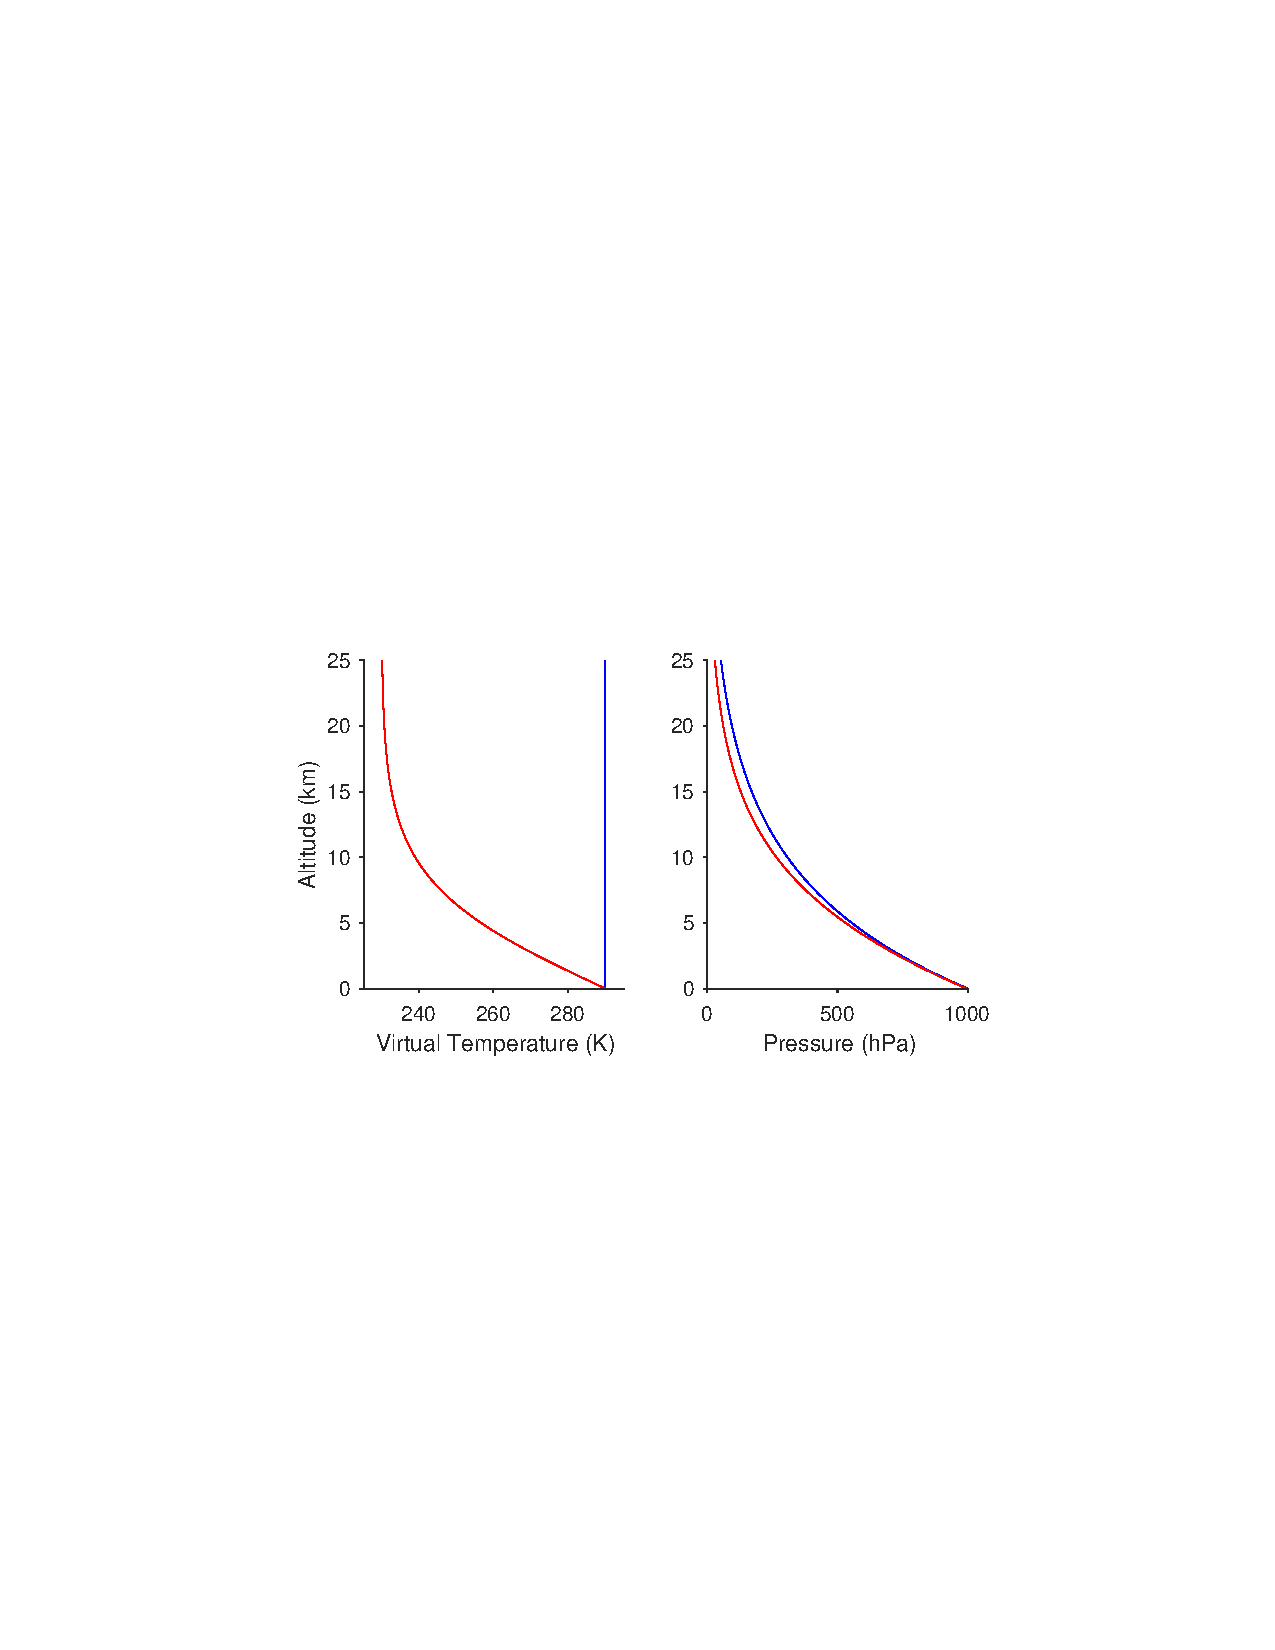
\includegraphics{figures/hydrostatic_state.pdf}
    \caption{(a) An isothermal temperature profile (blue) and a temperature profile \eqref{e:ref_temperature} (red) with surface temperature $T_{\mathrm{sfc}} = 300~\mathrm{K}$, ``stratospheric'' temperature $T_{\min} = 200~\mathrm{K}$, and ``tropospheric'' temperature lapse rate $\Gamma = 6.5~\mathrm{K~km^{-1}}$---values roughly representative of Earth's tropical atmosphere. (b) The corresponding hydrostatically balanced pressure profiles \eqref{eq:hydro_pressure_iso} and \eqref{eq:hydro_pressure_lapse}, with $p_{\mathrm{MSLP}} = 10^5~\mathrm{Pa}$.}
    \label{f:hydrostatic_state}
\end{figure}
The temperature is constant and equal to $T_{\min}$ above $z_t$. See Fig.~\ref{f:hydrostatic_state}a for an example. The resulting temperature profile is a rough approximation of a tropospheric temperature profile with lapse rate $\Gamma$ and a ``tropopause'' at height $z_t$, overlain by a ``stratosphere'' with constant temperature $T_{\min}$. For $\Gamma = g/c_{pd}$, the ``tropospheric'' temperature profile is dry adiabatic. 

\section{Pressure}

We obtain the pressure $p(z)$ consistent with the temperature profile $T(z)$ by combining hydrostatic balance ($\partial_z p(z) = - \rho g$) with the ideal gas law ($p=\rho R_d T$, neglecting the effect of any moisture on the gas constant), giving
\begin{equation}\label{eq:hydro_pressure}
p(z) = p_{\mathrm{MSLP}} \exp\left(-\int_0^z \frac{dz}{H(z)} \right).
\end{equation}
Here,
\begin{equation}
H(z)  = \frac{R_d T(z)}{g}
\end{equation}
is the scale height, and we chose for the pressure $p(0)$ at height $z=0$ the mean sea-level pressure $p_{\mathrm{MSLP}}$, a model parameter. 

It helps here to distinguish the cases of an isothermal atmosphere and of an atmosphere with nonzero lapse rate:
\begin{itemize}
\item \textbf{Isothermal Atmosphere ($\Gamma = 0$, $T_{\mathrm{sfc}} \ge T_{\min}$).} 
In this case, the pressure becomes 
\begin{equation}\label{eq:hydro_pressure_iso}
    p(z) = p_{\mathrm{MSLP}} \exp \left(-\frac{z}{H_{\mathrm{sfc}}} \right), \qquad H_{\mathrm{sfc}} = \frac{R_d T_{\mathrm{sfc}}}{g} = \mathrm{const}.
\end{equation}
See See Fig.~\ref{f:hydrostatic_state}b (blue line) for an example.

\item \textbf{Nonzero Lapse Rate ($\Gamma \ge 0$, $T_{\mathrm{sfc}} \ge T_{\min}$).}
Integrating the general expression \eqref{eq:hydro_pressure} for the hydrostatic pressure for a temperature profile \eqref{e:ref_temperature} with nonzero lapse rate yields
\begin{equation}\label{eq:hydro_pressure_lapse}
p(z) = p_{\mathrm{MSLP}} \times
\begin{cases}
\left(1 - \frac{\Gamma z}{T_{\mathrm{sfc}}} \right)^{g/(R_d \Gamma)} & \text{for } z \le z_t, \\[1.5ex]
  \left(\frac{T_{\min}}{T_{\mathrm{sfc}}} \right)^{g/(R_d \Gamma)}
 \exp  \left(-\frac{z - z_t}{H_{\min}} \right) & \text{for } z\ge z_t, 
\end{cases}
\end{equation}
where 
\begin{equation}
H_{\min} = \frac{R_d T_{\min}}{g}
\end{equation}
is the ``stratospheric'' scale height. See See Fig.~\ref{f:hydrostatic_state}b (red line) for an example. (The expression \eqref{eq:hydro_pressure_lapse} for nonzero lapse rate converges to the expression \eqref{eq:hydro_pressure_iso} for zero lapse rate in the limit $\Gamma \to 0$, as can be verified by L'H{\^o}pital's rule.)
\end{itemize}

\section{Density}
 
Given the temperature $T(z)$ and hydrostatic pressure $p(z)$, the reference density $\rho(z)$ follows from the ideal gas law as
\begin{equation}\label{eq:hydro_density}
    \rho(z) = \frac{p(z)}{R_d T(z)}.
\end{equation}

\section{Specific Humidity}

And the total specific humidity $q_t(z)$ for a given relative humidity, temperature $T(z)$, and density $\rho(z)$ is
\begin{equation}
    q_t(z) = \mathrm{RH} \, q_v^*\bigl( T(z), \rho(z) \bigr),
\end{equation}
where $q_v^*(T, \rho)$ is the saturation specific humidity \eqref{eq:sat_shum}. Corresponding to $\mathrm{RH} < 1$, we set the condensate specific humidities to zero ($q_l = q_i = 0$).

\section{Energy}

From the above quantities, we can compute the specific internal energy $I$ using Eq.~\eqref{eq:total_internal_energy} and with that the total specific energy $e^{\mathrm{tot}} = I + \Phi$ corresponding to a state of rest ($\vec{u}=0$). This completes the specification of the model state.

\section{Noise}

It is common to add a small amount of random noise, e.g., to the initial density at the surface, to break the symmetry of the initial state and allow three-dimensional instabilities to develop. A typical standard deviation of such noise may be 1\% of $\rho(0)$.

\chapter{Abstraction of Model Formulation}\label{s:abstract_model_formulation}

To describe the methods used to solve the governing equations numerically, let us write the equations in the compact form 
\begin{equation}\label{e:eom_compact}
\diff{\vec{Y}}{t}  =  - \nabla \cdot \Fvector + \vec{\mathcal{S}}(\vec{Y}),
\end{equation}
where $\vec{Y}$ is the \emph{state} vector, $\partial\vec{Y}/\partial t$ is the \emph{tendency} of the state vector, $\Fvector$ is the \emph{flux} vector, and $\vec{\mathcal{S}}(\vec{Y})$ are \emph{sources}. 

\section{State}

The state vector consists of components
\begin{equation}\label{e:state}
\vec{Y}=\left( \begin{array}{c}
\rho \\
\rho\vec{u} \\
\rho e^{\mathrm{tot}}\\
\rho q_k\\
\rho q_{p,i}\\
\rho \chi_j
\end{array}
\right).
\end{equation}
Here, $q_k$ represents the suspended water specific humidities $q_t$, $q_l$, and/or $q_i$ (total water and cloud condensate, if used); $q_{p,i}$ are the precipitation specific humidities, with the index $i$ labeling different precipitation species (rain, snow, graupel etc.); and $\chi_j$ are the scalar concentrations (e.g., mass of different aerosol species, chemical constituents etc.\ per unit mass of moist air). In some model configurations (e.g., when we include atmospheric chemistry), we may want to have $O(100)$ of these scalars, meaning that the state vector can consist of hundreds of components.

\section{Fluxes}\label{sec:fluxes}

The flux $\Fvector=\Fadv + \Pvector +  \Fdiff + \Frad + \Ffall$ consists of advective fluxes, pressure terms, diffusive fluxes, radiative fluxes, and sedimentation/precipitation fluxes. The diffusive components $\Fdiff$ are proportional to gradients of state variables, so that $\nabla \cdot \Fdiff$ contains elliptic operators. These are treated separately numerically from the non-diffusive fluxes, which do not contain gradients. Because the boundary conditions on advective and other non-diffusive fluxes generally differ, it is also useful to distinguish advective fluxes $\Fadv$, pressure terms $\Pvector$, and the other non-diffusive fluxes due to radiation $\Frad$ and sedimenting condensate and falling precipitation $\Ffall$. 

\subsection{Advective Fluxes}

The advective flux is generally of the form ``$\rho \times \mathrm{scalar} \times \vec{u}$,'' where $\vec{u}$ is the advective velocity of the working fluid. For the state vector \eqref{e:state}, it is 
 \begin{equation}
 \label{e:adv_flux}
 \Fadv=\rho \left( \begin{array}{c}
 \vec{u} \\
 \vec{u} \otimes \vec{u} \\
 e^{\mathrm{tot}} \vec{u}\\
q_k \vec{u}\\
q_{p,i} \vec{u} \\
\chi_j \vec{u}
\end{array}
\right).
 \end{equation}

\subsection{Pressure Terms}

The pressure terms in the momentum and energy equations can also be written in flux form,
\begin{equation}
\Pvector = \left( \begin{array}{c}
\vec{0} \\
p \vec{I}_3 \\
p \vec{u} \\
\vec{0} \\
\vec{0} \\
\vec{0} 
\end{array}
\right).
\end{equation}
Because pressure in a fluid is adjusted by sound waves, which are the fastest modes, the pressure terms are associated with the fastest time scales. 

\subsection{Diffusive Fluxes}

 The diffusive component takes the form 
 \begin{equation}
 \Fdiff=\left( \begin{array}{c}
 \rho\vec{d}_{q_t} \\
 \rho\vec{\tau} + \rho\vec{d}_{q_t} \otimes \vec{u}\\
 \vec{u} \cdot \rho\vec{\tau} + \rho (\vec{J} + \vec{D}) \\
\rho\vec{d}_{q_k}\\
\rho \vec{d}_{q_{p, i}}\\
\rho \vec{d}_{\chi_j}
\end{array}
\right).
\label{eq:diff_flux}
\end{equation}
where the water flux $\vec{d}_{q_t}$ is defined in \eqref{eq:sgs-shum-flux}, the momentum flux $\vec{\tau}$ in \eqref{e:sgs_momentum_flux}, the total enthalpy flux $\vec{J} + \vec{D}$ in \eqref{e:SGS_energy_flux}, the fluxes of the water components $\vec{d}_{q_k}$ are defined in \eqref{e:water_diffusion}, the fluxes $\vec{d}_{q_{p, i}}$ of the precipitation components in \eqref{eq:sgs-precip-flux}, and the fluxes $\vec{d}_{\chi_j}$ of tracers in \eqref{eq:sgs-tracer-flux}.


\subsection{Other Non-diffusive Fluxes}

The other non-diffusive fluxes include source terms (e.g., radiation) that can be written in flux form but that are not proportional to gradients of state variables, as well as the sedimentation and precipitation fluxes involving the sedimentation and fall velocities $w_l$, $w_i$, and $w_p$ (approximately terminal velocity) of condensate and falling precipitate:
\begin{equation}
\Frad = 
\left( \begin{array}{c}
\vec{0} \\
\vec{0} \\
\rho \vec{F}_R \\
\vec{0} \\
\vec{0} \\
\vec{0} 
\end{array}
\right), \qquad
\Ffall = 
- \left( \begin{array}{c}
\rho q_{c} w_{c} \vec{k}  \\
q_c w_c \vec{k} \otimes \rho \vec{u}  \\
\rho W_c \vec{k} \\
\rho q_{k} w_{k} \vec{k}  \\
\rho q_{p,i} w_{p, i} \vec{k} \\
\rho \chi_{i} w_{\chi, i} \vec{k} 
\end{array}
\right).
\label{eq:ndf_flux}
\end{equation}
The fall velocities $w_l$, $w_i$, and $w_{p, i}$ are point-wise functions of the specific humidities, the environmental density $\rho$, and of other microphysical parameters that determine the size distribution of cloud condensate particles and falling hydrometeors. The radiative energy flux $\vec{F}_R$ is included here because it is not diffusive in character. In climate models, it generally is approximated as vertical and hence is one-dimensional, like the precipitation flux. Therefore, \emph{the divergence of these two fluxes is a one-dimensional (vertical) divergence}. \hl{[TODO in code: Do we have this implemented as a vertical divergence only?]}

\section{Sources}

The right-hand side of the balance law \eqref{e:eom_compact} has the source-sink terms
\begin{multline}
\Source(\vec{Y})= 
 \left( \begin{array}{c}
 -\rho C(q_t \rightarrow q_p) \\
  -\rho \nabla\Phi - 2 \vec{\Omega} \times \rho\vec{u}  + \rho \vec{F}_u \\
 \rho Q - \sum_{j\in\{v,l,i\}} (I_j + \Phi)  \rho C(q_j \rightarrow q_p) + \rho \vec{u} \cdot \vec{F}_u - M \\
\rho C(q_p \rightarrow q_k) + \rho \sum_j \rho C(q_j \rightarrow q_k) \\
\rho \sum_k C(q_k \rightarrow q_{p, i}) - \rho \sum_j C(q_{p, i} \rightarrow q_{p, j})\\
\rho \mathcal{S}_{\chi_i}
\end{array}
\right)
\label{eq:source}
\end{multline}
where $C(q_j \rightarrow q_k)$ represents the conversion of the generic specific humidity $q_j$ to $q_k$ ($k, j \in \{v, l, i\}$), $C(q_p \rightarrow q_k)$ represents the conversion of all precipitation specific humidities $q_p$ to $q_k$, and $C(q_{p, i} \rightarrow q_{p, j})$ represents conversion among precipitation species $q_{p, i}$ and $q_{p, j}$. 

\section{Boundary Conditions}

At rigid boundaries with normal $\vec{n}$, the normal component of the advective velocity $\vec{u} \cdot \vec{n}$ vanishes, and so do the normal components of all advective fluxes $\Fadv$. Normal components of diffusive fluxes, on the other hand, generally do not vanish (e.g., there are diffusive energy and momentum fluxes across the lower boundary, as discussed in section~\ref{sct:bc}). For these, Neumann boundary conditions apply. In some circumstances (e.g., simulations with prescribed sea surface temperature), we will also need to specify Dirichlet boundary conditions. 

Thus, generally, we want vanishing normal flux components at rigid boundaries, and Dirichlet conditions on state variables and/or Neumann conditions on diffusive flux components.

\chapter{Numerical Methods}\label{sec:numerical_methods}

\hl{[Numerical Methods have moved to a separate document in CLIMA-Numerics]}

\chapter{Benchmark Cases}

Here we describe a suite of test cases for dry and moist atmospheres, and for coarse-resolution global and higher-resolution limited-area model configurations. 

\hl{STILL INCOMPLETE}

\section{Held-Suarez (1994) Dry GCM Benchmark}

\citet{Held94} describe a simple and widely used setup for testing dry dynamical cores of GCMs. This setup is usually used to focus on statistically steady states (reached after about 100--400~days of spinup) but also lends itself to the study of the time-dependent evolution of Rossby waves and baroclinic instability. In this benchmark calculation, vertical SGS fluxes are usually set to zero; however, horizontal diffusion (or hyperdiffusion) is needed to damp the enstrophy cascade. 

\subsection{Initial Condition}

The initial condition for the Held-Suarez benchmark is an isothermal atmosphere at rest, with $T(t=0) = 300~\mathrm{K}$. Hydrostatically balanced initial density and pressure fields are calculated from the initial temperature according to section~\ref{s:initial_conditions}, and some small random perturbations are added to the density field to break the symmetry of the initial state and allow 3D baroclinic waves to develop. Baroclinic waves develop within a few simulated days in this benchmark calculation, and they begin to equilibrate after around 20--30~days. 

\subsection{Boundary Conditions}

The lower boundary condition is free-slip and thermally insulating, with no evaporation. That is, \emph{all} diffusive fluxes at the lower boundary (see section~\ref{s:bottom_bc}) are taken to be zero (if they are not already taken to be zero throughout the atmosphere, which is common in the Held-Suarez benchmark). With the vanishing surface fluxes, there is no need to specify a surface temperature.

\subsection{Sources}

\subsubsection{Momentum} 

Bottom drag in this benchmark calculation is modeled as a momentum sink in the lower part of the atmosphere, which is a function of velocity $\vec{u}$ and pressure $p$. The momentum sink takes the form of linear Rayleigh drag
\begin{equation}
    \vec{F}_u = -k_v(\sigma) \vec{u},
\end{equation}
where the drag coefficient decays away from the surface:
\begin{equation}
    k_v(\sigma) = k_f \max \left( 0, \frac{\sigma - \sigma_b}{1-\sigma_b} \right).
\end{equation}
Here,
\[
\sigma = \frac{p}{p_{\mathrm{MSLP}}}
\]
is a normalized pressure. (Usually, $\sigma$ is taken to be normalized by the temporally and spatially varying surface pressure $p_s$. But we can simplify this to a constant pressure.) \hl{[It would be good at some point to change this to the actual surface pressure, but this is not important now.]} The two parameters are
\begin{itemize}
    \item $\sigma_b = 0.7$: vertical extent of drag layer
    \item $k_f = 1~\mathrm{day^{-1}}$: drag coefficient at the surface
\end{itemize}.

\hl{Note that the momentum source appears in the momentum and energy equations. In hydrostatic models, the Rayleigh drag only acts on the horizontal velocity components and is zero in the vertical. Would that be easy to implement for us? Otherwise, also damping vertical velocities is ok for now, but it may need to strongly distorted upwelling and subsidence.}

\subsubsection{Heating/cooling}

Radiative heating/cooling is represented by linear relaxation of temperatures toward a radiative-equilibrium state with temperature \hl{[Note that here $p/p_{\mathrm{MSLP}}$ should be this, with a constant pressure for normalization. So generally, this is not equal to $\sigma$ above; it is only with the simplified $\sigma$ above.]}
\begin{multline}
    T_{\mathrm{eq}} = \max \\
    \left\{ T_{\mathrm{top}}, \left[ T_{\max} - (\Delta T)_y \sin^2 \phi - (\Delta \theta)_z \log\left(\frac{p}{p_{\mathrm{MSLP}}}\right) \cos^2 \phi \right]
    \left( \frac{p}{p_{\mathrm{MSLP}}} \right)^{\kappa} \right\}.
\end{multline}
Here, $\phi$ is latitude, $\kappa = R_d/c_{pd}$ is the adiabatic exponent, and the default values of the parameters are:
\begin{itemize}
    \item $T_{\mathrm{top}} = 200~\mathrm{K}$: temperature at model top
    \item $T_{\max} = 315~\mathrm{K}$: near-surface temperature at equator
    \item $(\Delta T)_y = 60~\mathrm{K}$: pole-equator temperature difference in radiative equilibrium
    \item $(\Delta \theta)_z = 10~\mathrm{K}$: static stability in background state.
\end{itemize}

Relaxation of temperatures toward the background state on a timescale $k_T^{-1}$ implies a source in the energy equation that is a function of latitude $\phi$, pressure $p$, and temperature $T$:
\begin{equation}
    Q =  - c_{vd} k_T(\phi, p) (T - T_{\mathrm{eq}}).
\end{equation} 
The relaxation coefficient $k_T$ is taken to vary with latitude and normalized pressure $\sigma$ as
\begin{equation}
k_T(\phi, p) = k_a + (k_s - k_a) \max\left(0, \frac{\sigma - \sigma_b}{1-\sigma_b}\right) \cos^4 \phi ,
\end{equation}
where 
\begin{itemize}
    \item $k_a = (40~\mathrm{day})^{-1}$: relaxation coefficient in interior atmosphere
    \item $k_s = (4~\mathrm{day})^{-1}$: relaxation coefficient  at equator near the surface.
\end{itemize}
The interior relaxation timescale $k_a^{-1}$ controls the timescale over which they flow equilibrates to a statistically steady state

\subsection{SGS Fluxes}

In global models with a stratified atmosphere, large-scale turbulence with Rossby waves usually dominates the kinetic energy of the flow. The large-scale flow is primarily rotational and horizontal. SGS dissipation primarily needs to absorb the cascade of enstrophy (vorticity variance) to small scales. This is usually accomplished by horizontal hyperdiffusion.

Hence, the SGS mixing needs to be strongly anisotropic, e.g., as outlined in section~\ref{s:anisotropic_SGS_mixing}.

\section{2D Rising Thermal Bubble (Robert 1993)}
\label{2dRTBtest}
\cite{robert1993} describes a test of a thermal bubble rising in an isentropic environment. The atmosphere is initially neutrally stratified with uniform potential temperature $\theta_0 = 303~\mathrm{K}$. The initial state is in hydrostatic equilibrium, so that the pressure decreases with $z$ as
\begin{equation}
\label{pressureDistrib}
p = p_{0}\left(1-\frac{g}{c_p{\theta_{0}}}z\right)^{c_p/R}.
\end{equation}
The domain is $\Omega=[-5000~\mathrm{m},5000~\mathrm{m}]\times[0,10000~\mathrm{m}]$. The flow is triggered by a Gaussian-shaped potential temperature perturbation with a flat region at the center, defined as
\begin{equation}
 \Delta\theta = \left\{ \begin{array}{ll}
 \theta_c & \text{if } r \leq a\\
 \theta_c e^{-(x - a)^2/\sigma^2} & \text{if } r > a\\
\end{array} \right.
\label{eq:robertIni}
\end{equation}
where $r = \sqrt[]{(x-x_{c})^{2} + (z-z_{c})^{2}}$, $(x_c,z_c) = (500,260)\,\mathrm{m}$, $a=50~\mathrm{m}$, $\sigma = 100~\mathrm{m}$, and $\theta_c=0.5~\mathrm{K}$.

\begin{figure}[htbp]
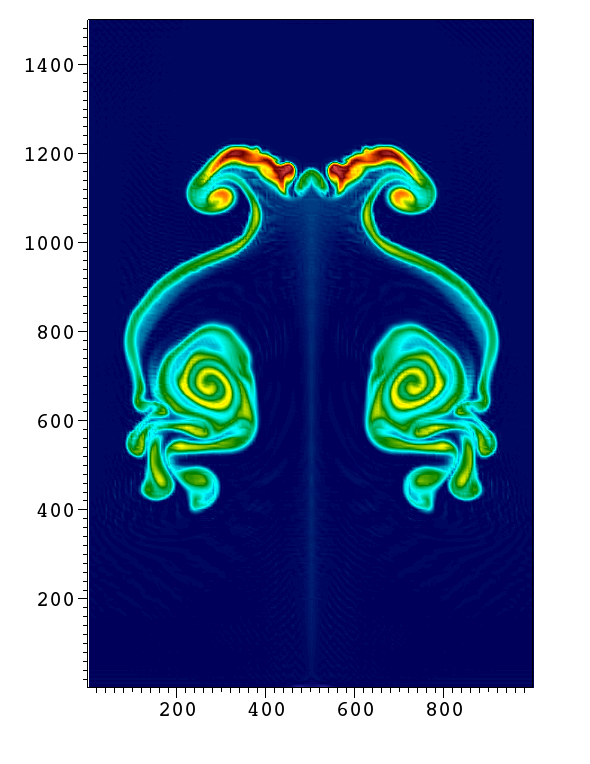
\includegraphics[width=\textwidth]{figures/RTB-Robert--smgo-5mX5m-1080s0000.png}
\caption{2D rising thermal bubble (Robert, 1993) stabilized via a constant coefficient Smagorinsky-Lilly SGS: Potential temperature, $\theta$, at $t=1080\,\mathrm{s}$. Grid resolution: $\Delta x = \Delta z = 5\,\mathrm{m}$.}
\label{fig:benchmarks/robert5msmago}
\end{figure}

\section{2D Density Current}
This test is described in \cite{strakaWilhelmson1993}. It consists of a flow that is triggered by the cold perturbation of a neutrally stratified atmosphere at initially uniform potential temperature $\theta_0 = 300$ K
and in hydrostatic equilibrium such that the pressure decreases with $z$ as:
\begin{equation}
\label{pressureDistrib2}
p = p_{0}\left(1-\frac{g}{c_p{\theta_{0}}}z\right)^{c_p/R}.
\end{equation}
The domain $\Omega=[-25600,25600]\times[0,6400]\,\mathrm{m}^2$.
The perturbation is linear and defined as
\begin{equation}
 \Delta\theta = \left\{ \begin{array}{ll}
 0 & \mathrm{if } r > 1\,{\mathrm K}\\
 0.5 \theta_c \left(1 + \cos(\pi r) \right) \leq 1\,{\mathrm K}\\
\end{array} \right.
\label{eq:robertIni2}
\end{equation}
where $r = \sqrt[]{(x-x_{c})^2/r_x^{2} + (z-z_{c})^{2}/r_z^2}$, $(x_c,z_c) = (0,4000)\,\mathrm{m}$, $(r_x, r_z) = (4000, 2000)\,\mathrm{m}$ and $\theta_c=-15$ K. The fully developed density current at $t=900\,\mathrm{s}$ simulated with a grid effective resolution of $25$ m in both spatial directions is shown in Figure \ref{fig:benchmarks/dc25msmago}.

\begin{figure}[htbp]
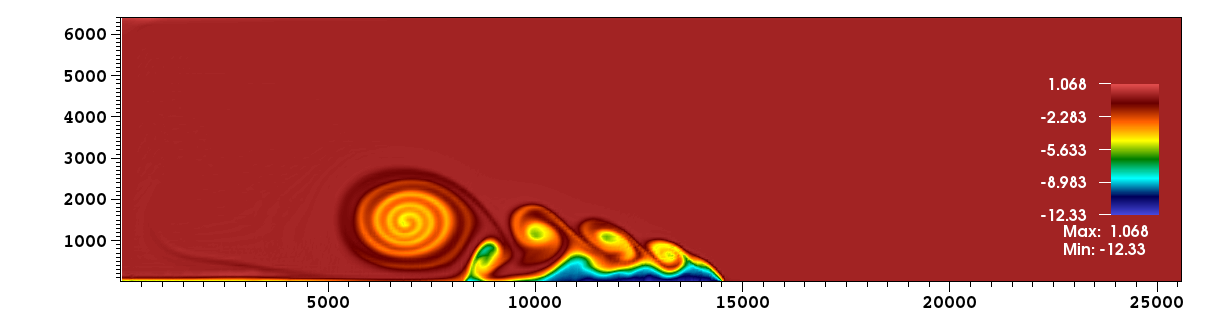
\includegraphics[width=1.2\textwidth]{figures/DC-smgo-25mx25m-900s0000.png}
\caption{2D density current stabilized via a constant coefficient Smagorinsky-Lilly SGS. Potential temperature, $\theta$, at $t=900\,\mathrm{s}$ (top) and at $t=1200\,\mathrm{s}$ (bottom). Grid resolution: $\Delta x = \Delta z = 25\,\mathrm{m}$.
}
\label{fig:benchmarks/dc25msmago}
\end{figure}


%%
\section{Rising Thermal Bubble in a Saturated Atmosphere}
\label{rtb3D}
The moist dynamics is tested by means of the saturated rising bubble test described in \cite{Pressel15a}. The initial conditions are setup as follows:

\begin{itemize}
\item Initialize dry atmosphere with uniform background $\theta_{ref} = 320$ K
\item Add thermal perturbation $\Delta \theta$ of radius $r=2$ km
\item Set a uniform total mixing ratio $q_t = 0.0192 \,\mathrm{kg/kg}$ and $q_l = q_i = 0.0\,\mathrm{kg/kg}$
\item Calculate the gas constants for moist air: 
\[\begin{array}{lcl}
R_{gas} &=& {\tt MoistThermodynamics.gas\_constant\_air(q_t, q_l, q_i)}\\
c_v     &=& {\tt MoistThermodynamics.cv\_m(q_t, q_l, q_i)}\\
c_p     &=& {\tt MoistThermodynamics.cp\_m(q_t, q_l, q_i)}\\
\end{array}
\]
\item  Compute $\theta$, $\rho$, and $T$ as if the background were dry:\\
    \[ \begin{array}{lcl}
  \theta &=& \theta_{ref} + \Delta\theta\\
 \pi & =& 1 - gz/(c_p\theta)\\
 \rho & = & p_0/(R_{gas}\theta)\pi^{c_v/R_{gas}}\\
 T   & = &\pi \theta
\end{array}\]

\item Add the contribution of moisture to the internal energy and recalculate $T$ and $P$, and obtain $e^{\rm tot}$ using the following {\tt MoistThermodynamics} functions:
\[\begin{array}{lcl}
I &=& {\tt MoistThermodynamics.internal\_energy(T + T_0, q_t, q_l, q_i)}\\
T &=& {\tt MoistThermodynamics.air\_temperature(I, q_t, q_l, q_i)}\\
P &=& {\tt MoistThermodynamics.air\_pressure(T - T_{ref} , \rho, q_t, q_l, q_i)}\\
e^{\rm tot} &=& {\tt MoistThermodynamics.total\_energy(0.5\|{\bf u} \|^2, gz, T, q_t)}
\end{array}\]
\end{itemize}

%%
\section{Dynamics and Chemistry of Marine Stratocumulus: DYCOMS RF01}

\subsection{Initial Condition}

\cite{Stevens05a} provide the following initial distributions of liquid water potential temperature,
\begin{equation}\label{eq:dycoms1}
\theta_l(z) = 
    \begin{cases}
    289.0\;\mathrm{K} & z\leq z_i,\\
    297.5 + (z - z_i)^{1/3}\;\mathrm{K}& z > z_i,
    \end{cases}
\end{equation}
and total specific humidity, 
\begin{equation}\label{eq:dycoms2}
q_t(z) = 
    \begin{cases}
    q_{t,0} & z\leq z_i,\\
    1.5\;\mathrm{g/kg} & z > z_i.
    \end{cases}
\end{equation}
Here, $z_i$ is the initial cloud top set to $z_i=840\,\mathrm{m}$. \cite{Stevens05a} state that ``modeling groups were also asked to standardize their thermodynamic calculations'' so that the initial state corresponds to a cloud layer between 600 and 800~m with liquid water specific humidity
\begin{equation}\label{eq:dycoms3}
q_l(z) = 
    \begin{cases}
    0 & z\leq 600~\mathrm{m},\\
    0.45\frac{{}z - 600~\mathrm{m}}{z_i - 600~\mathrm{m}}\;\mathrm{\frac{g}{kg}}   & 600~\mathrm{m} < z \leq z_i,\\
    0 & z > z_i.\\
    \end{cases}
\end{equation}
With our thermodynamics and standard thermodynamical constants, we obtain such a cloud layer if we choose the initial total specific humidity in the mixed layer to be $q_{t,0} = 8.1\;\mathrm{g/kg}$, which is slightly lower than the DYCOMS default value of $9\;\mathrm{g/kg}$. (An alternative to modifying the initial $q_{t,0}$ would be to adjust, e.g., the latent heat of vaporization or the vapor pressure at the triple point to obtain the desired cloud layer with $q_{t,0} = 9\;\mathrm{g/kg}$.)

To specify the thermodynamic state completely, we additionally need to specify an initial density. We do so by first specifying an initial pressure
\[
p_0(z) = p_{s} \exp(-z/H), \qquad H = \frac{R_m T_{BL}}{g},
\]
where $R_m = R_m(q_t, q_l)$ is the gas constant for moist air, $T_{BL} = 285.0~\mathrm{K}$ is an average boundary-layer temperature, and $p_s = 1.0178\times 10^{5}~\mathrm{Pa}$ is the surface pressure, with surface density $\rho_s = 1.22~\mathrm{kg/m^3}$ and surface temperature $T_s = p_s/(\rho_s R_{m,s})$. Consistent with the Boussinesq or anelastic approximation used in most DYCOMS simulations, we calculate thermodynamic quantities with this reference pressure $p_0(z)$. We use the linearized expression for the liquid-water potential temperature,
\begin{equation}
    \label{eq:betts1973}
    \theta_l = \theta \left(1 - \frac{L_{v,0} q_l}{c_{pm} T} \right) = \theta - \frac{L_{v,0} q_l}{c_{pm} \Pi_0},
\end{equation}
where $\theta = T/\Pi_0$, and 
\[
\Pi_0 = \left( \frac{p_0(z)}{p_{s}} \right)^{R_d/c_{pd}}
\]
is evaluated with the pressure profile $p_0(z)$. This can be solved for temperature as a function of height $z$,
\[
T = \Pi_0 \theta_l + \frac{L_{v,0} q_l}{c_{pm} \Pi_0},
\]
given $\theta_l(z)$, $q_l(z)$, and $\Pi(z)$. Density is then obtained from the ideal gas law as
\[
\rho(z) \approx \frac{p_0(z)}{R_m T(z)},
\]
thus completely specifying the initial state. 

The initial state of all the quantities described above are plotted in Figure \ref{dycomsInitFig}
\begin{figure}
    \centering
	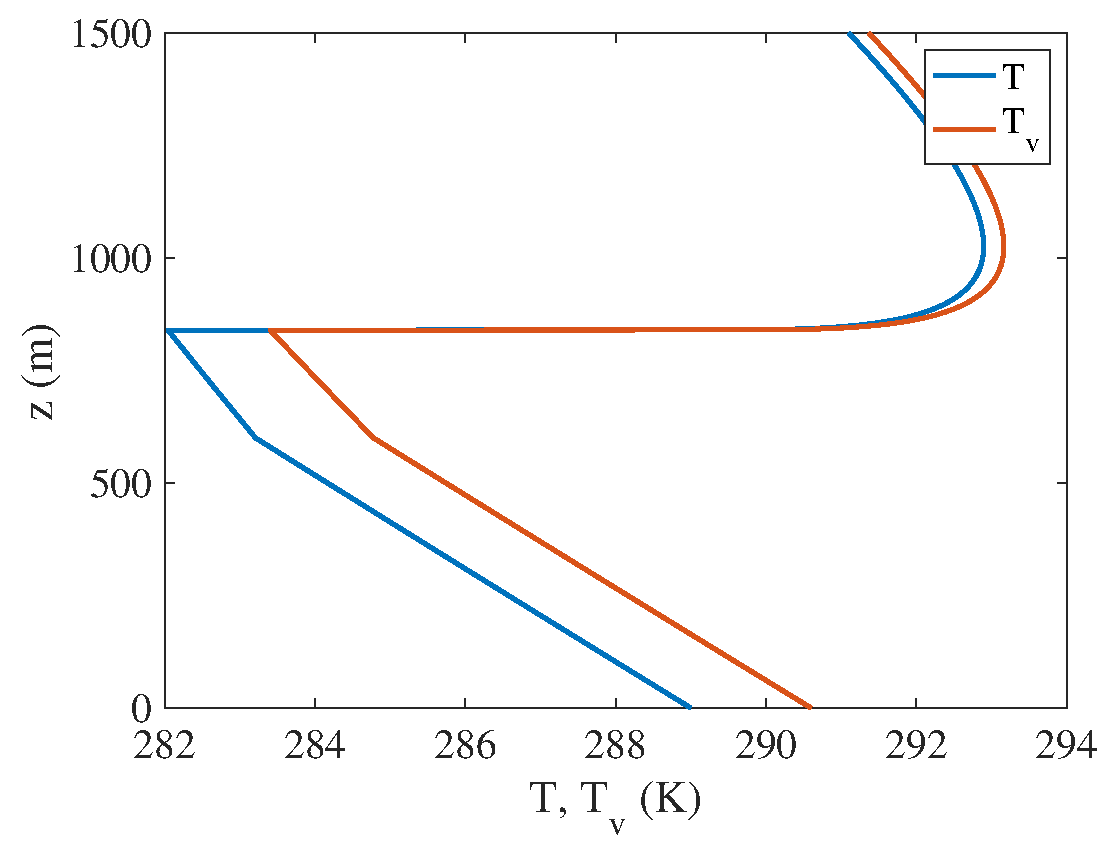
\includegraphics[width=0.49\textwidth]{figures/dy_tempe.eps}
	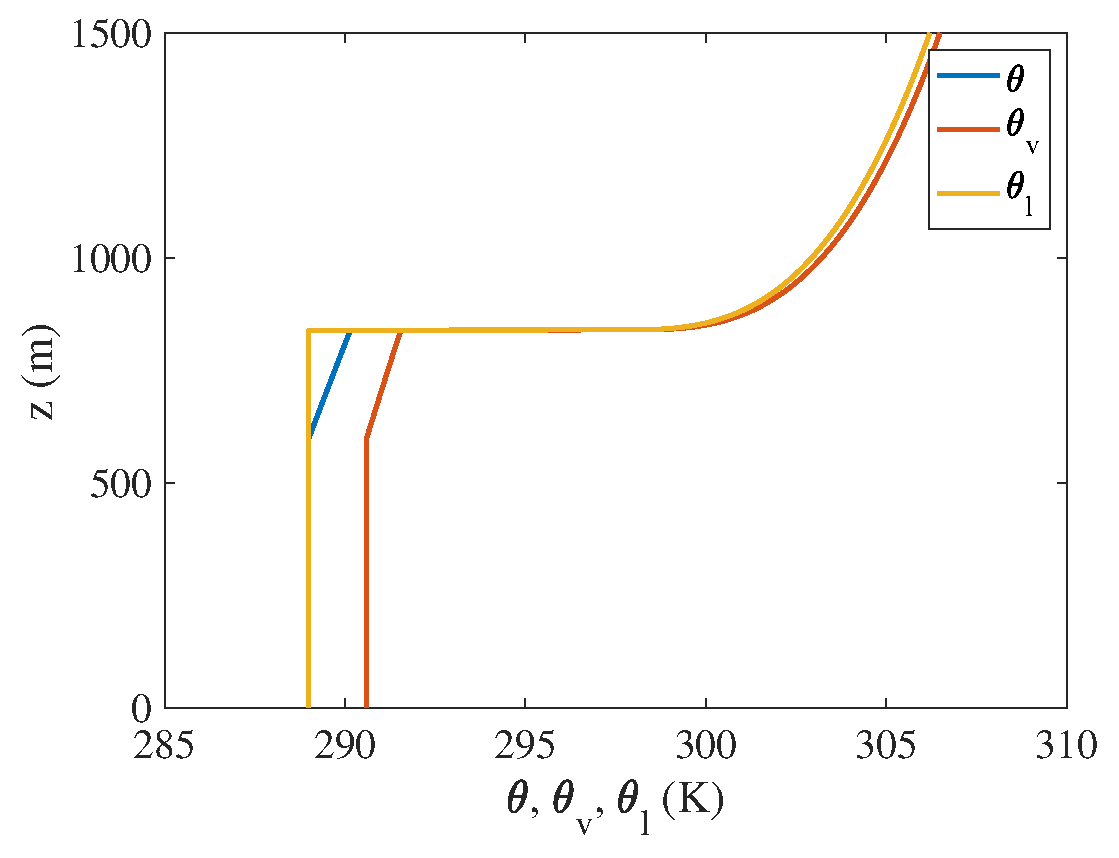
\includegraphics[width=0.49\textwidth]{figures/dy_pot_temp.eps}
	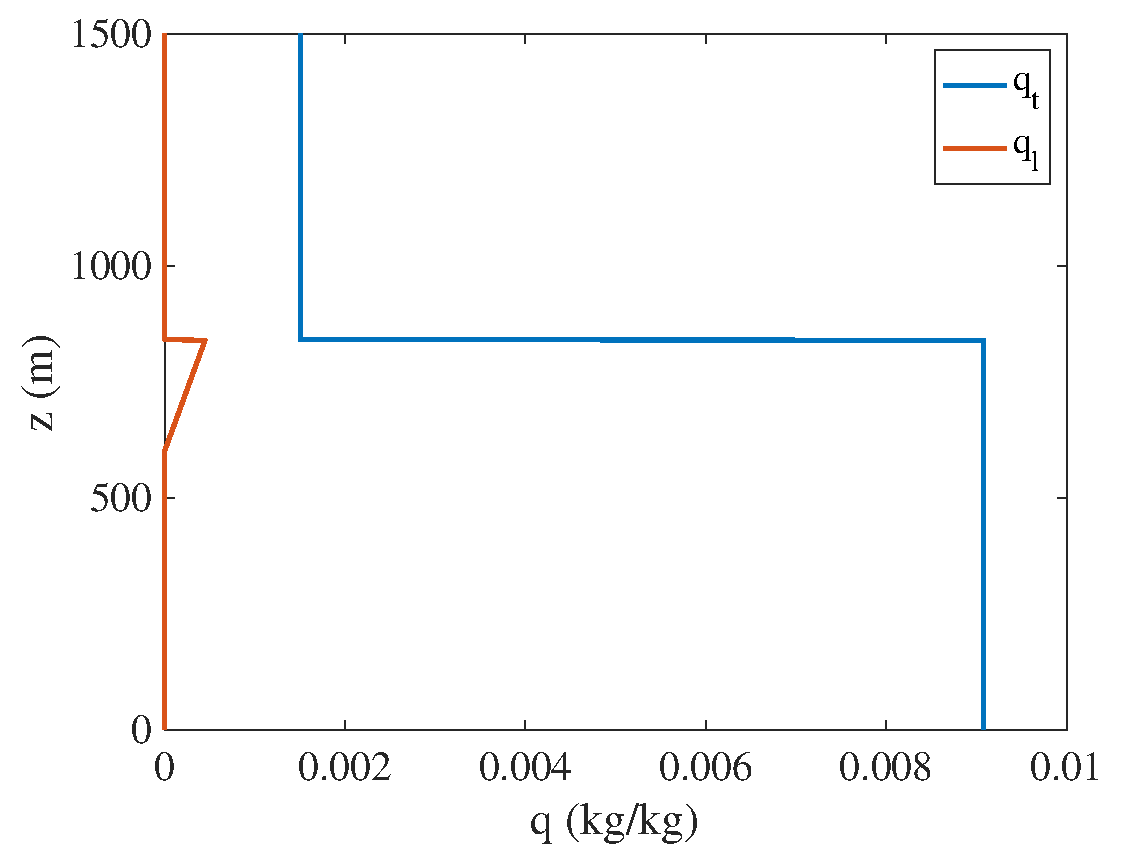
\includegraphics[width=0.49\textwidth]{figures/dy_mixing_ratios.eps}
	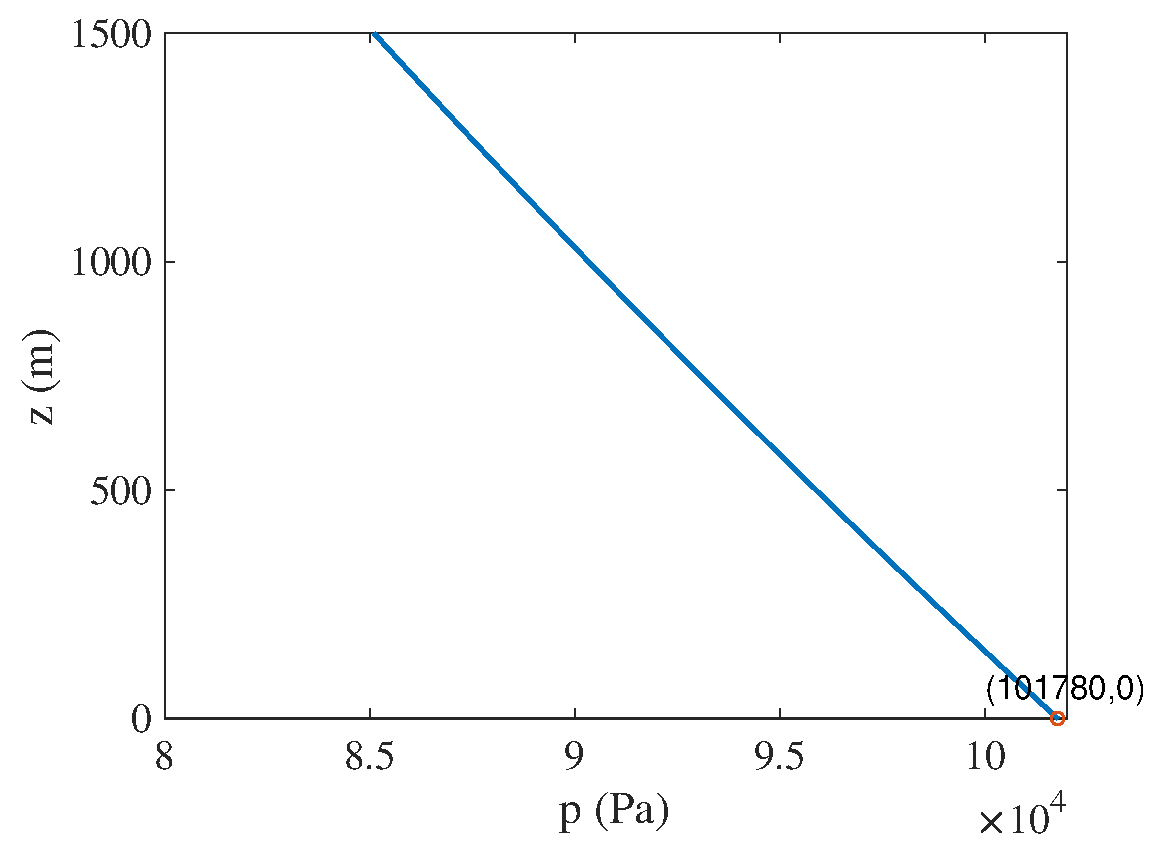
\includegraphics[width=0.49\textwidth]{figures/dy_press.eps}
	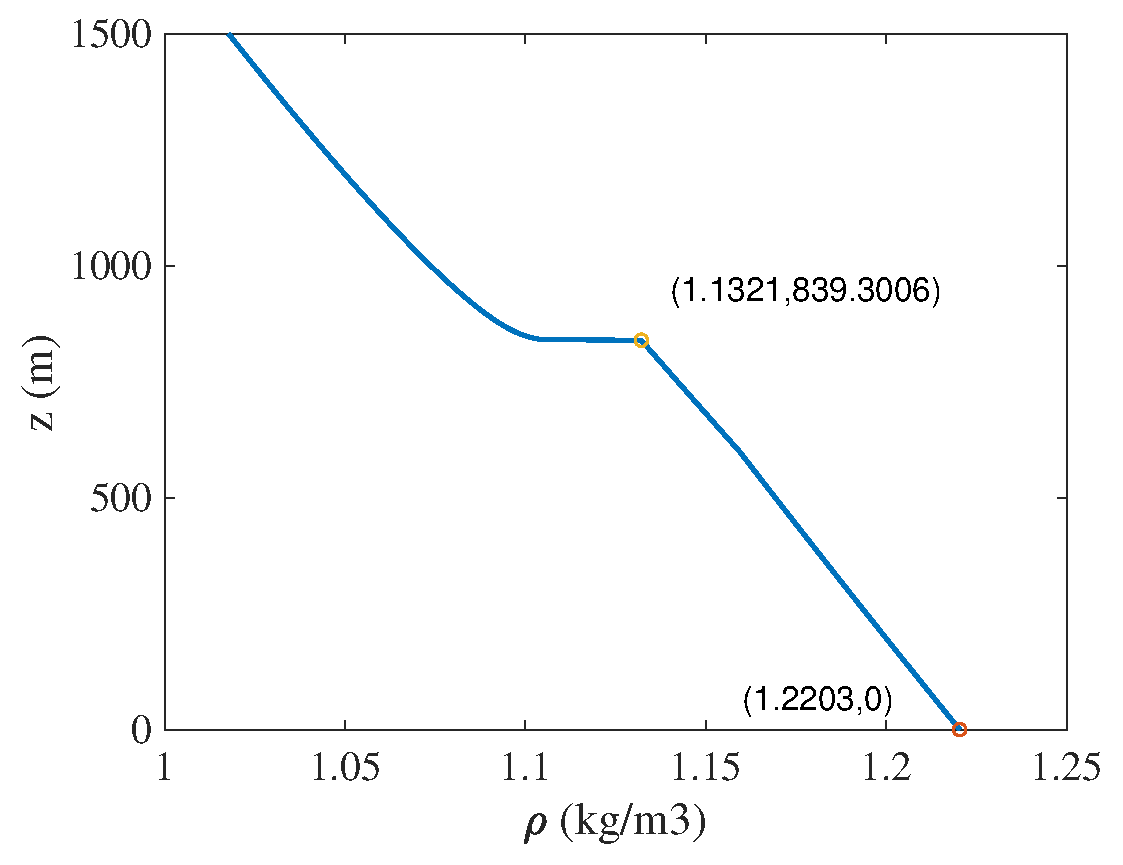
\includegraphics[width=0.49\textwidth]{figures/dy_densi.eps}
	%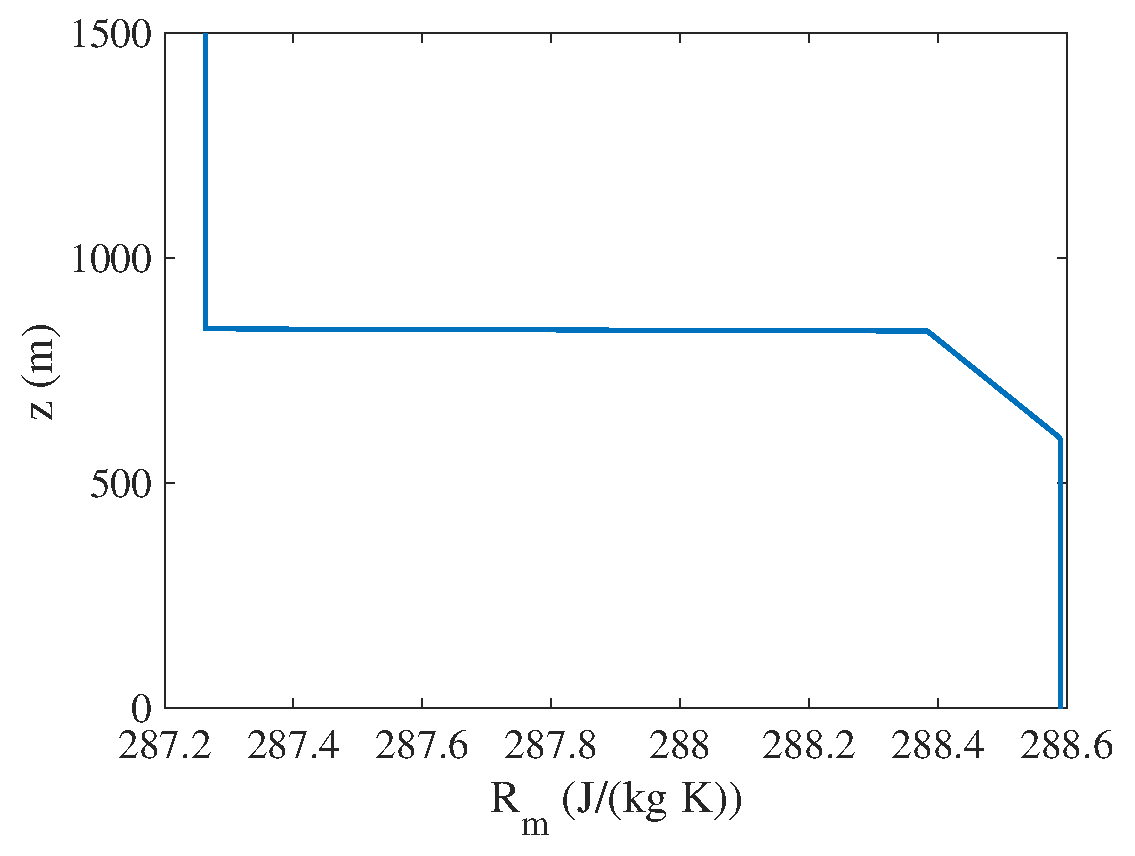
\includegraphics[width=0.49\textwidth]{figures/dy_Rm.eps}
	%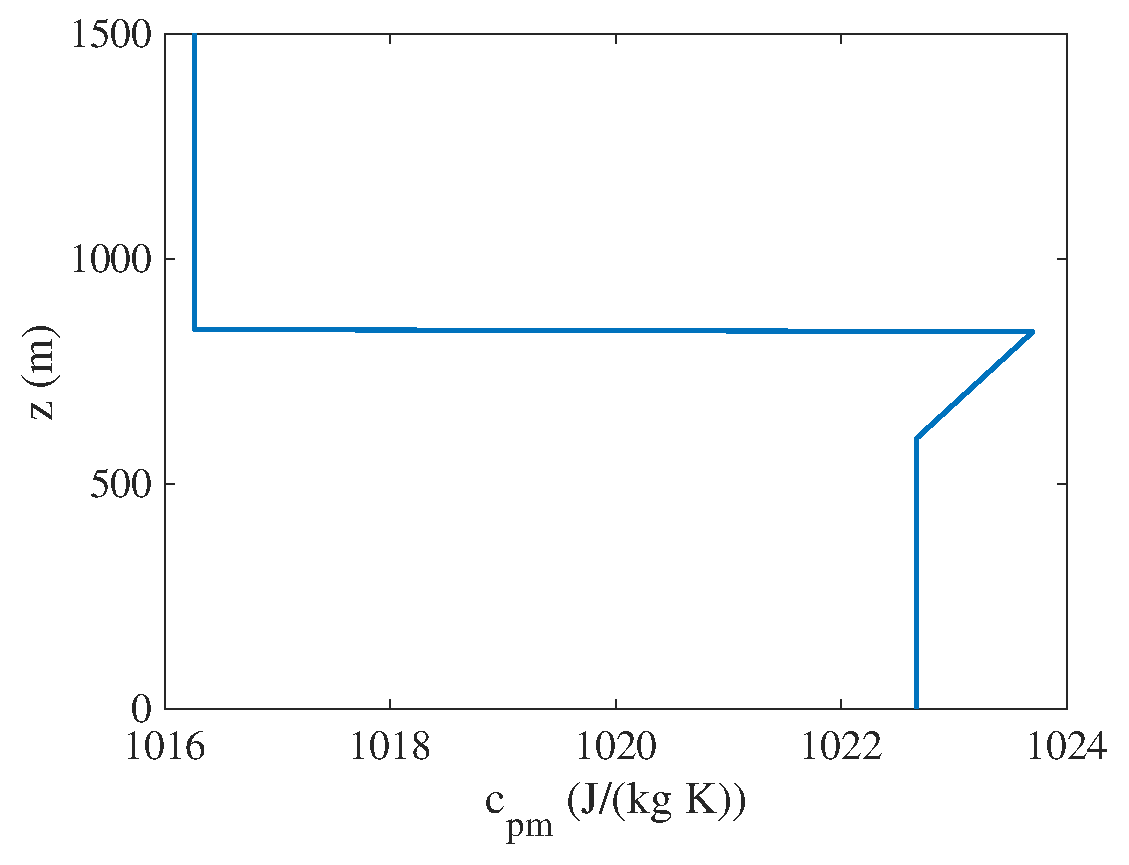
\includegraphics[width=0.49\textwidth]{figures/dy_cpm.eps}
      \caption{Dycoms: initial states of $T, T_v, \theta, \theta_v, \theta_l, q_t, q_l, p, \rho$.}
\label{dycomsInitFig}
\end{figure}

\subsection{Boundary Conditions}

The bottom boundary conditions for DYCOMS are prescribed energy and water fluxes and a drag law for momentum, as described in section~\ref{s:bottom_bc}. The prescribed fluxes at the surfaces are
\begin{itemize} 
\item Sensible heat flux $\mathrm{SHF} = \vec{n} \cdot (\rho \vec{J}_{\mathrm{sfc}}) = 15\,\mathrm{W/m^2}$
\item Latent heat flux $\mathrm{LHF} = \vec{n} \cdot (\rho \vec{D}_{\mathrm{sfc}}) = 115\,\mathrm{W/m^2}$
\item Energy flux $\vec{n} \cdot \rho (\vec{J}_{\mathrm{sfc}} + \vec{D}_{\mathrm{sfc}}) = \mathrm{LHF + SHF} = 130\,\mathrm{W/m^2}$
\item Evaporation $E \approx \mathrm{LHF}/L_{v,0}$
\end{itemize}

\subsection{Sources}

\subsubsection{Radiative cooling}
Radiative cooling is imposed through the simple model described by \cite{Stevens05a}. It specifies the vertical radiative energy flux $\Frad = F_R \vec{k}$ (part of the non-diffusive energy fluxes \eqref{eq:ndf_flux}) as
\begin{equation}
    \label{e:radiativeStevens05}
    F_{R}({\bf x}, t) = F_0{\rm e}^{-Q(z,\infty)} +
    F_1{\rm e}^{-Q(0, z)} +
    \rho_i c_{pd} D \alpha_z\frac{(z-z_i)^{4/3}}{4} + z_i(z - z_i)^{1/3}
\end{equation}
where 
\begin{equation}
    Q(a,b) = \kappa\int_{a}^{b}\rho\,q_l\,dz.
\end{equation}
The following parameters are used:
$F_0=70\,\mathrm{W\,m^{-2}}$, $F_1=22\,\mathrm{W\,m^{-2}}$, $\kappa=85\,\mathrm{m^2\,kg^{-1}}$, $\alpha_z=1\,\mathrm{m^{-4/3}}$. The parameter $D=3.75\times 10^{-6}\,\mathrm{s^{-1}}$ gives the large-scale divergence, which also enters the dynamical equations as an additional advection term.  

\subsubsection{Large-scale subsidence}

A large-scale subsidence velocity $W=-Dz$ is imposed and is added to the internally generated vertical velocity $w$ in all governing equations. 

\subsection{SGS Fluxes}

The interaction of the resolved flow with SGS fluxes is crucial for a successful simulation of stratocumulus \citep{Pressel17a}. If there is too much spurious mixing across the sharp inversion interface, the clouds dissipate because too much dry air from above the clouds is mixed into the clouds. Hence, it is important to use SGS schemes that limit mixing near the stable inversion interface.

\section{3D Squall Line}
\label{sq3D}
The three-dimensional simulation of a squall line is defined in the domain 
$80\times 80\times20\,\mathrm{km}^3$. 
The initial background state is given by the sounding of \cite{gabersekGiraldoDoyle2012}.
To initiate the vertical transport of water vapor to a level of condensation (and hence trigger a cloud formation, the initial background is forced by a temperature anomaly $\theta'$ $3$ K warmer than the surrounding environment. 

A stretched grid along $z$ is used to make the resolution higher in the lower atmosphere where convection is triggered.
The domain is crossed by a horizontal wind along the x-direction with a $12\,\mathrm{m\,s^{-1}}$ shear at $z=2000\,\mathrm{m}$.
A no-slip condition is applied on the surface boundary while periodic boundaries are defined along $x$ and $y$. 
To damp the vertically propagating gravity ways triggered by the cloud formation, a Rayleigh absorbing layer is applied at the higher layers of the atmosphere.
The cloud first forms at approximately 500 s, and is fully develop after 4500 s. 
An instantaneous view of the precipitating squall line is shown in Figure \ref{fig:benchmarks/squall1}. 

\begin{figure}[htbp]
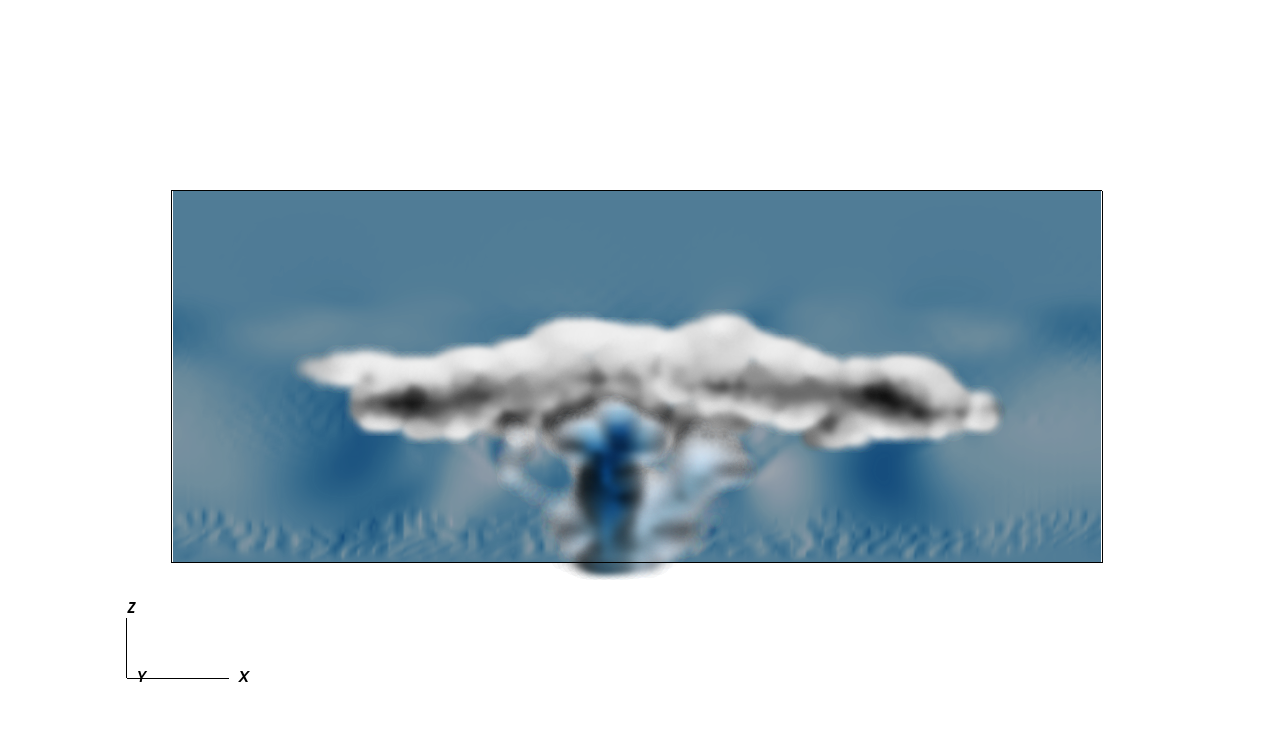
\includegraphics[width=1.2\textwidth]{figures/squall_working_warm_rain_frontal_view0028.png}
\caption{Front view of a fully developed squall line with precipitating rain. }
\label{fig:benchmarks/squall1}
\end{figure}

\section{External Soundings}
External soundings can be read into the code for initialization purposes. The sounding requires the format reported in Table \ref{tab:DeltaDefinitionsTable}.

\begin{table*}[t]
\centering
{\footnotesize
\caption[short]{Structure of sounding files for simulation initialization.}
\label{tab:DeltaDefinitionsTable}
\begin{tabular*}{\textwidth}{ @{\extracolsep{\fill}} llllll}
\hline
\hline
z (m) & $\theta_v$ (K) & $q_{tot}$ $\rm {kg/kg}$ & $u$ (m/s) & $v$ (m/s) & p (Pa)\\
0 & 300 & 14  & -2 & 0 & 100000\\
... & ... & ...  & ... & ... & ...\\
\hline
\hline
\end{tabular*}
}
\end{table*}

\chapter{Input/Output}
\section{Inputs}

\section{Outputs}
\section{Three dimensional fields}


\section{Diagnostics}

A Reynolds decomposition is applied to all quantities for which statistics are computed. For a given quantity $a$, it is split into a mean value, $<a>$  (in either time or space) and a fluctuation, $a'$, around it such that $a' = a - <a>$, where the space or time averaging is simply:

\begin{equation}
    \langle a \rangle = \frac{1}{N} \sum_{i=1}^N a_i
\end{equation}
where $N$ indicates either the number of time or space samples. \hl{An ensemble average should also be added at some point}.

For space averaging, data are first interpolated onto an auxiliary Cartesian mesh with equally spaced nodes. The auxiliary mesh is usually coarser than the solution mesh.
The spatial means are computed across two-dimensional slices of the auxiliary mesh at each vertical level  \hl{to be done}.

The statistics listed in Table \ref{tab:stats} are calculated during the simulation at a regular interval defined by the user. 

\begin{table*}[t]
\centering
{\footnotesize
\caption[short]{Structure of sounding files for simulation initialization.}
\label{tab:stats}
\begin{tabular*}{\textwidth}{ @{\extracolsep{\fill}} lccc}
\hline
\hline
Vertical velocity variance & & &$<w' w'>$\\
Third moment of vertical velocity & & &$<w'w'w'>$\\
Vertical heat flux & & &$<w' \theta'>$\\
Vertical water vapor flux & & &$<w' q_v'>$\\
...\\
\hline
\hline
\end{tabular*}
}
\end{table*}

The velocity two-point correlation is used to extract the energy spectrum as follows:

\begin{equation}
    E(k) = \int \Phi_{ij}dV
\end{equation}

The energy spectrum is calculated by means of the i of the velocity spectrum The velocity spectrum is first calculated by means of the Fourier transform of the correlation 

\section{File formats}
Three dimensional data are written to disk in parallel (one file per processor \hl{Jeremy, please confirm}) using the {\it Visualization Toolkit} (VTK) format (\cite{vtkWeb}). The user defines the writing interval.
VTK should soon be replaced by the HDF5 file format (\cite{hdf5web}).
Statistical quantities are now written out to ASCII files which are read and plotted via a set of Python scripts (under construction).


%-------Bibliography
\bibliographystyle{agufull08}
\bibliography{Giraldo_refs,CLIMA-refs}

\end{document}
